\published{Geophysics, 84(1), F1-F15, (2019)}

\title{CuQ-RTM: A CUDA-based code package for stable and efficient Q-compensated reverse time migration}

\renewcommand{\thefootnote}{\fnsymbol{footnote}}

\author{Yufeng Wang\footnotemark[1], Hui Zhou\footnotemark[1], Xuebin Zhao\footnotemark[1], Qingchen Zhang\footnotemark[2], Poru Zhao\footnotemark[3], Xiance Yu\footnotemark[3], and Yangkang Chen\footnotemark[4]}
\address{
\footnotemark[1] State Key Laboratory of Petroleum Resources and Prospecting \\
China University of Petroleum \\
Fuxue Road 18th\\
Beijing, China, 102200 \\
\footnotemark[2]Research Center for Computational and Exploration Geophysics\\
 State Key Laboratory of Geodesy and Earth’s Dynamics\\
  Institute of Geodesy and Geophysics\\
   Chinese Academy of Sciences\\
    Wuhan, Hubei Province, China, 430077\\
\footnotemark[3]
China National Petroleum Corporation\\
Beijing, China. \\
\footnotemark[4]
School of Earth Sciences\\
Zhejiang University\\
Hangzhou, Zhejiang Province, China, 310027\\
yangkang.chen@zju.edu.cn 
}

\lefthead{Wang et al, 2019}
\righthead{CUDA-based Q-RTM}

\maketitle

\begin{abstract}
Reverse time migration (RTM) in attenuating media should take the absorption and dispersion effects into consideration. The latest proposed viscoacoustic wave equation with decoupled fractional Laplacians (DFLs) facilitates separate amplitude compensation and phase correction in $Q$-compensated RTM ($Q$-RTM). However, intensive computation and enormous storage requirements of $Q$-RTM prevent it from being extended into practical application, especially for large-scale 2D or 3D case. The emerging graphics processing unit (GPU) computing technology, built around a scalable array of multithreaded Streaming Multiprocessors (SMs), presents an opportunity for greatly accelerating $Q$-RTM by appropriately exploiting GPU's architectural characteristics. We present the cu$Q$-RTM, a CUDA-based code package that implements $Q$-RTM based on a set of stable and efficient strategies, such as streamed CUFFT, checkpointing-assisted time-reversal reconstruction (CATRC) and adaptive stabilization. The cu$Q$-RTM can run in a multi-level parallelism (MLP) fashion, either synchronously or asynchronously, to take advantages of all the CPUs and GPUs available, while maintaining impressively good stability and flexibility. We mainly outline the architecture of the cu$Q$-RTM code package and some program optimization schemes. The speedup ratio on a single GeForce GTX760 GPU card relative to a single core of Intel Core i5-4460 CPU can reach above 80 in large-scale simulation. The strong scaling property of multi-GPU parallelism is demonstrated by performing $Q$-RTM on a Marmousi model with one to six GPU(s) involved. Finally, we further verify the feasibility and efficiency of the cu$Q$-RTM on a field data set. The ``living'' package is available from GitHub at \url{https://github.com/Geophysics-OpenSource/cuQRTM}, and peer-reviewed code related to this article can be found at \url{http://software.seg.org/2019/0001}.
\end{abstract}

\section{Introduction}

Seismic wave absorption and dispersion, resulting from the presence of intrinsic anelasticity in subsurface media, has been considered one of the most important factors degrading the quality of seismogram and decreasing the resolution of migrated images, which affects the reliability of seismic interpretation \citep{Wang2004Seismic, carcione2007wave, wang2018L}. Many models have been proposed to characterize this frequency-dependent attenuation, which can be roughly classified into two categories: mechanical models and mathematical models. The former includes standard spring-pot models such as the Maxwell body, Kelvin-Voigt model, standard linear solid (SLS) model \citep{carcione2007wave, mainardi2010fractional}, their generalizations such as the generalized Maxwell body (GMB) and generalized Zener body (GZB) \citep{moczo2005rheological, cao2014equivalence}, and their fractional extensions such as the fractional Kelvin model (FKM), fractional Zener model (FZM) \citep{rossikhin2010application, nasholm2013fractional}. Generally, the attenuation of seismic waves appears to be adequately modeled by a power law \citep{strick1967determination, szabo1994time, szabo1995causal} or linear dependence on frequency over a finite bandwidth (a special case of power-law attenuation with a power of 1) \citep{mcdonal1958attenuation, futterman1962dispersive, kjartansson1979constant}. Therefore, another category of models is established on the assumption of power-law attenuation, which includes the Kolsky-Futterman model \citep{kolsky1956lxxi, futterman1962dispersive}, the power-law model and Kjartansson's constant-$Q$ model \citep{kjartansson1979constant}. 

The attenuation models mentioned above are designed for mathematically characterizing frequency-dependent attenuation effects of subsurface media and further paving the way to mitigate these effects during seismic wave propagation. Early attempts to compensate for the $Q$ effect (attenuation and dispersion effects) are mostly conducted in the framework of one-way wave-equation migration (OWWEM) \citep{Dai1994Inverse, mittet1995prestack, Wang2004Seismic, mittet2007simple, zhang2012compensation}. In recent years, $Q$-RTM has received increasing attention from the geophysical community \citep{Causse2000Viscoacoustic, Zhang2010Compensating, Zhu2014Q, Li2016Efficient, sun2016q, guo2016comparison, wang2018adaptive}, which generalizes acoustic RTM by considering viscoacoustic propagation and compensating amplitude loss and phase distortion during source and receiver wavefields extrapolation.  \cite{Zhu2014Modeling} proposed a novel viscoacoustic wave equation with decoupled fractional Laplacians (DFLs) which separately dominate amplitude attenuation and phase dispersion, and they further applied this viscoacoustic wave equation in RTM so as to improve the resolution and quality of the image \citep{Zhu2014Q}. This decoupled viscoacoustic wave equation is attractive for $Q$-RTM due to its flexibility for separate amplitude compensation and phase correction, which can be achieved by simply reversing the absorption proportionality coefficient in sign while leaving the equivalent dispersion parameter unchanged \citep{Treeby2010Photoacoustic, Zhu2014Q}. 

Although the basic paradigm of $Q$-RTM has been well-established in recent years, there are still some problems and limitations in the process of the implementation, i.e., intensive computation, huge storage requirements and frequent disk I/O, and the difficult issue of stability. The emerging graphics processing unit (GPU) computing technology, built around a scalable array of multithreaded Streaming Multiprocessors (SMs), presents an opportunity for accelerating $Q$-RTM much further by appropriately exploiting the GPU's architectural characteristics \citep{tan2016faster, farquhar2016gpu}. As a booming technology, the GPU computing technology has been widely applied into seismic modeling \citep{micikevicius20093d, zhang2014time}, imaging \citep{zhang2009accelerating, foltinek2009industrial, liu2012fourier, Liu20133D, Yang2014RTM}, and inversion \citep{shin20143d, Yang2015A}. In this chapter, we present a CUDA-based code package named cu$Q$-RTM, which aims to tackle these problems so as to achieve an efficient, storage-saving and stable $Q$-RTM. Next, we will briefly introduce how cu$Q$-RTM is designed to deal with these challenges and then outline the architecture of the cu$Q$-RTM code package. 

Specifically, in order to avoid intensive computation, we implement $Q$-RTM in a multi-level parallel (MLP) fashion, either synchronously or asynchronously, to take advantage of all the CPUs and GPUs available. In the framework of cu$Q$-RTM, the basic forward and backward modeling modules, based on viscoacoustic wave equations with DFLs, are efficiently simulated using the Fourier pseudospectral method (PSM) \citep{Carcione2010A, Zhu2014Modeling, chen2016two}. Discrete Fourier transforms (DFTs) of complex wavefields are the most time-consuming parts of these modules. Fortunately, DFTs can be efficiently computed by calling the CUFFT library API \citep{guide2013cuda}, which provides a simple interface for computing parallel FFTs on the GPU, and a simple configuration mechanism called a plan that completely specifies the optimal plan of execution. The use of a CUFFT standard library brings two obvious benefits: the configuration mechanism allows us to create the plans once and execute the plans multiple times (at every time step of the iteration) without recalculation of the configuration. Every CUFFT plan can be associated with a specified CUDA stream. Streaming the CUFFT execution allows for potential overlap between transforms and memory copies and provides a balanced calculation load on each card of the GPUs. CUFFT library functions can only be executed on the device and called from the host, so we have to split my customized kernel functions into k-space components and x-space components. From the brief codes in Appendix A, one can clearly figure out how these components are interconnected.

Apart from the issue of intensive computation, extensive data storage and burdensome disk I/O are another two bottlenecks for conventional RTM, especially for CUDA-based RTM which demands frequent memory copying between host and device \citep{Liu20133D, Yang2014RTM}. In the past three decades, several wavefield reconstruction strategies have been developed to reach a reasonable compromise between the computer memory requirement and computational complexity, for example, reverse propagation coupled with effective boundary saving \citep{Yang2014RTM}, the optimal checkpointing scheme \citep{Griewank2000Algorithm, Symes2007Reverse}, and their combinations such as the time-reversal checkpointing method \citep{Anderson2012Time} and the checkpointing-assisted reverse-forward simulation (CARFS) method \citep{yang2016wavefield}. \cite{yang2016wavefield} proposed a novel viscoacoustic wavefield reconstruction algorithm referred as CARFS, which is implemented by monitoring the energy errors of the reconstruction, and taking it as a criterion to decide whether forward simulation or reverse simulation will be performed at the next time step. \cite{wang2017wavefield} proposed a robust viscoacoustic wavefield reconstruction scheme using time-reversal checkpointing (TRC) and k-space filtering (KSF). In this hybrid scheme, TRC serves as a time-domain regularization to eliminate accumulating errors by replacing the reconstructed wavefield with the stored wavefield at checkpoints, whereas KSF further suppresses high-wavenumber artifacts introduced during time-reversal reconstruction. In the cu$Q$-RTM package, we adopt the checkpointing-assisted time-reversal reconstruction (CATRC) scheme to reconstruct source wavefields, which combines the efficiency of reverse propagation and the stability of checkpointing. Unlike CARFS, the proposed CATRC scheme keeps the reconstruction errors within an acceptable range by imposing low-pass filtering on the time-reversal reconstructed wavefield so as to maintain a fixed recomputation ratio of two. 

Finally, amplitude compensation in $Q$-RTM suffers from numerical instability because of it boosts high-frequency noise arising from high-frequency noise in seismic data and numerical errors from the finite machine precision \citep{wang2009seismic, Zhu2014Q, yang2016wavefield, zhao2017method}. Therefore stabilization needs to be introduced either in the frequency or wavenumber domain \citep{Kalimeris2012Photoacoustic, Ammari2013Time}. Since the forward and backward modeling modules are simulated by PSM in cu$Q$-RTM, it is more natural to conduct stabilization in the wavenumber domain. In some literature concerning $Q$ compensation, high-frequency noises are suppressed by utilizing a low-pass Tukey filter with its cutoff frequency identified by the noise level of measured data \citep{Treeby2010Photoacoustic, Zhu2014Q,Li2016Efficient}. However, conventional time-invariant filtering fails to adapt with $Q$ distribution and compensation depth (travel time). \cite{wang2018adaptive} developed an adaptive stabilization for Q-RTM by analytically deriving k-space Green's functions for the constant-$Q$ wave equation with DFLs and its compensated equation, where the stabilization factor can be explicitly identified by the specified gain limit according to an empirical formula. In the provided package, we utilize the proposed adaptive stabilization method to deal with numerical instability in $Q$-RTM, which exhibits superior properties of time-variance and $Q$-dependence over conventional low-pass filtering. 

In this paper, we present an open-source code package cu$Q$-RTM, which overcomes several problems commonly existing in conventional $Q$-RTM such as intensive computation, data storage and numerical stability, by adopting stable and efficient strategies like streamed CUFFT, CATRC and adaptive stabilization. The general architecture of the cu$Q$-RTM code package consists of memory manipulation, modules, kernels, and multi-level parallelism. Each component plays an indispensable role in GPU-CPU cooperative computing. We further demonstrate the validity and efficiency of cu$Q$-RTM with both synthetic and field examples. 

\section{Overview of $Q$-RTM}

In this section, we first review the general principle of $Q$-RTM in the framework of viscoacoustic wave equation with DFLs, which includes viscoacoustic propagation, compensation, and imaging. Besides that, two stable and efficient strategies, CATRC and adaptive stabilization, are also provided to improve the computation and stability performance of $Q$-RTM.

\subsection{Propagation, compensation, and imaging}

The viscoacoustic wave equation with DFLs was first proposed by \cite{Zhu2014Modeling} to characterize frequency-dependent attenuation and dispersion separately, which can be written as
\begin{equation}  
\left\{  
             \begin{array}{lr}  
             \dfrac{1}{c^2}\dfrac{\partial^2p}{\partial t^2}(\mathbf{x},t)-\eta(-\nabla^2)^{\gamma+1}p(\mathbf{x},t)-\tau \dfrac{\partial}{\partial t}					
             (-\nabla^2)^{\gamma+\frac{1}{2}}p(\mathbf{x},t) = \delta(\mathbf{x}_s)f(t),  &  \\  
             p(\mathbf{x},t)=\dfrac{\partial p}{\partial t}(\mathbf{x},t)=0,   \qquad \mathbf{x} \in \Omega, t<0 , & 
             \end{array}  
\right.  
\label{eq:forward}
\end{equation} 
where $\Omega$ is a bounded domain in $d$-dimensional space $\mathbb{R}^d$, $\mathbf{x}_s$ denotes the source position, and $f(t)$ is the point source signature enforced at $\mathbf{x}_s$. The dimensionless parameter $\gamma=\mathrm{arctan}(1/\pi Q)$ ranges within $[0, 1/2)$, and $c^2=c_0^2\mathrm{cos}^2(\pi \gamma /2)$, where $c_0$ is the velocity model defined at the reference frequency $\omega_0$. The proportionality coefficients of two fractional Laplacians, separately representing dispersion and absorption, are given by $\eta =-c_0^{2\gamma}\omega_0^{-2\gamma} \mathrm{cos}(\pi \gamma)$ and $\tau=-c_0^{2\gamma-1}\omega_0^{-2\gamma}\mathrm{sin}(\pi \gamma)$. Equation \ref{eq:forward} seems to be attractive for $Q$-RTM owing to its flexibility for separately compensating amplitude loss and correcting phase distortion. \cite{Treeby2010Photoacoustic} and \cite{Zhu2014Q} stated that attenuation compensation based on this equation can be achieved by reversing the absorption proportionality coefficient in sign but leaving the equivalent dispersion parameter unchanged. My latest work (in Chapters 4 and 5) has analytically proved that Green's function of equation \ref{eq:forward} is exponentially decreasing, whereas reversing the absorption proportionality coefficient in sign signifies replacing the Green's function with a phase-conjugated Green's function that is exponentially increasing \citep{wang2018adaptive, wang2017k}. 

The novel paradigm of $Q$-RTM first proposed by \cite{Zhu2014Q}, where the source wavefield $p_s(\mathbf{x},t)$ and receiver wavefield $p_r(\mathbf{x},t)$ are compensated during forward extrapolation and time-reversal extrapolation simultaneously, coupled with a zero-lag crosscorrelation imaging condition, has proven to be a promising approach for generating high-resolution images and high-fidelity amplitude reflectors. Following the spirit of \cite{Treeby2010Photoacoustic} and \cite{Zhu2014Q}, the $Q$-compensated source wavefield $p_s(\mathbf{x},t)$ is the solution of the following equation:
\begin{equation}  
\left\{  
             \begin{array}{lr}  
             \dfrac{1}{c^2}\dfrac{\partial^2p_s}{\partial t^2}(\mathbf{x},t)-\eta(-\nabla^2)^{\gamma+1}p_s(\mathbf{x},t)+\tau \dfrac{\partial}{\partial t}					
             (-\nabla^2)^{\gamma+\frac{1}{2}}p_s(\mathbf{x},t) = \delta(\mathbf{x}_s)f(t),  &  \\  
             p_s(\mathbf{x},t)=\dfrac{\partial p_s}{\partial t}(\mathbf{x},t)=0,   \qquad \mathbf{x} \in \Omega, t<0, & 
             \end{array}  
\right.  
\label{eq:Qpforward}
\end{equation} 
and the $Q$-compensated receiver wavefield $p_r(\mathbf{x},t)$ satisfies the following equation
\begin{equation}
\left\{  
            \begin{array}{lr}
			\dfrac{1}{c^2}\dfrac{\partial^2p_r}{\partial t^2}(\mathbf{x},t)-\eta(-\nabla^2)^{\gamma+1}p_r(\mathbf{x},t)+\tau \dfrac{\partial}{\partial t}		
			(-\nabla^2)^{\gamma+\frac{1}{2}}p_r(\mathbf{x},t) = \delta(\mathbf{x}_r)g(\mathbf{x},T-t), &  \\ 
			g(\mathbf{x},t)=p(\mathbf{x},t), \qquad \mathbf{x} \in \mathbf{x}_r, t \in [0,T], & 
            \end{array}  
\right.  
\label{eq:Qpbackward}
\end{equation} 
where $\mathbf{x}_r$ denotes the receiver positions, $g(\mathbf{x},t)$ stands for the recorded seismic data at $\mathbf{x}_r$, which are reversed in time and enforced as the Dirichlet boundary condition. Finally, we realize $Q$-RTM via the following zero-lag crosscorrelation imaging condition:
\begin{equation}
I(\mathbf{x})= \int_0^T p_s(\mathbf{x},t) p_r(\mathbf{x},t) dt.
\label{eq:ic}
\end{equation}
However, an inevitable issue imposed by the crosscorrelation algorithm is that the forward wavefields need to be accessible at every time step \citep{Anderson2012Time, yang2016wavefield}. Saving all forward wavefields requires tremendous memory and frequent disk I/O, which makes it impractical for large-scale 2D or 3D RTM \citep{Symes2007Reverse, Tan2014Reducing}, especially for CUDA-based RTM that demands data transfer between host and device \citep{Yang2014RTM}. 



\subsection{CATRC}

In order to relieve extensive data storage and burdensome disk I/O and thus reach a reasonable compromise between the computer memory requirement and computational complexity, we propose an efficient wavefield reconstruction strategy named CATRC, which combines the efficiency of reverse propagation and the stability of checkpointing. Therefore source wavefields used in imaging condition in equation \ref{eq:ic} can be well-reconstructed during time-reversal simulation. Here we denote the reconstructed wavefields as $q(\mathbf{x},t)$, which is the solution of
\begin{equation}  
\left\{  
             \begin{array}{lr}  
             \dfrac{1}{c^2}\dfrac{\partial^2q}{\partial t^2}(\mathbf{x},t)-\eta(-\nabla^2)^{\gamma+1}q(\mathbf{x},t)-\tau \dfrac{\partial}{\partial t}			
             (-\nabla^2)^{\gamma+\frac{1}{2}}q(\mathbf{x},t) = \delta(\mathbf{x}_{\partial \Omega})h(\mathbf{x},T-t),  &  \\  
             h(\mathbf{x},t)=p_s(\mathbf{x},t),   \qquad \mathbf{x} \in \partial \Omega, t \in [0,T] , &  \\
             q(\mathbf{x},t)=p_s(\mathbf{x},t),  \qquad  t \in \big \{C_i \mid i \in [0, N_c-1]\big \} \bigcup \big \{T, T-\Delta t\big \}, &
             \end{array}  
\right.  
\label{eq:catrc}
\end{equation} 
where $\partial \Omega$ is the boundary of space $\Omega$, $h(\mathbf{x},t)$ are forward wavefields distributed on $\partial \Omega$, which are reversed in time and enforced as the Dirichlet boundary condition for source wavefield reconstruction. $C_i$ denotes a checkpoint, and $N_c$ is the number of checkpoints. According to equation \ref{eq:catrc}, the implementation of CATRC can be briefly summarized as two processes. Firstly, we compute forward wavefield $p_s(\mathbf{x},t)$ by solving the compensated viscoacoustic wave equation in \ref{eq:Qpforward}, and we save the forward wavefield at the outermost layer boundary of the simulation domain at every time step. At the same time, we also save the complete forward wavefield $p_s(\mathbf{x},t)$ at the predefined checkpoints ($t \in C_i, i=0, \cdots , N_c-1$) and the last two time steps. The checkpoints can be equally distributed or logarithmically distributed \citep{Griewank2000Algorithm, Symes2007Reverse}. Next, we compute the backward wavefield $q(\mathbf{x},t)$ in reverse time (from $t=T$ to $t=0$) by solving the reconstructed viscoacoustic wave equation (equation \ref{eq:catrc}), and replacing the calculated backward wavefield $q(\mathbf{x},t)$ with the recorded forward wavefield $p_s(\mathbf{x},t)$ at checkpoints ($t \in C_i, i=N_c-1, \cdots , 0$).

It is remarkable that reconstruction by equation \ref{eq:catrc} is a mathematically stable process, given that the source wavefield is compensated while the reconstructed wavefield from boundary is attenuated. However, this stable reconstruction still suffers from insufficient accuracy due to the fact that we utilize PSM to solve equation \ref{eq:catrc} with only the recorded forward wavefield at the outermost layer boundary of simulation domain at every time step. This mismatch of simulation accuracy inevitably degrades the performance of the wavefield reconstruction. Fortunately, the time-reversal checkpointing scheme acts as a time-domain regularization that eliminates accumulating errors by replacing the reconstructed wavefield with the stored wavefield at checkpoints \citep{wang2017wavefield}.

\subsection{Adaptive stabilization}

Mathematically speaking, the compensated viscoacoustic wave equations \ref{eq:Qpforward} and \ref{eq:Qpbackward} are severely ill-posed due to the presence of the compensating term $+\tau \partial_t (-\nabla^2)^{\gamma+1/2} p(\mathbf{x},t)$. That is to say, amplitude compensation is a nonstationary process with energy exponentially amplified over travel time, which boosts high-frequency ambient noise and can even result in numerical instability. In the package, we apply an adaptive stabilization scheme for $Q$-RTM to suppress unwanted high-frequency artifacts, which is discussed in my previous work \citep{wang2018adaptive}. Here we briefly summarize the process.

I derive a k-space Green's function of equation \ref{eq:forward} by enforcing a point source at time $t=t_0$ and $\mathbf{x}=\mathbf{x}_s$. The time-space harmonic Green's function $G(\mathbf{k},\omega)$ is the solution of the following Helmholtz equation
\begin{equation}  
\left(\frac{\omega^2}{c^2}+\eta |\mathbf{k}|^{2\gamma+2}+i\omega\tau|\mathbf{k}|^{2\gamma+1}\right)G(\mathbf{k},\omega)=\frac{1}{(2\pi)^{d+1}}e^{-i \omega t_0} e^{i\mathbf{k} \mathbf{x}_s}.
\label{eq:kwgreen}
\end{equation} 
Solving for Green's function $G(\mathbf{k},\omega)$, applying $d+1$ dimensional inverse Fourier transformation, and then integrating the kernel function with respect to $\omega$ based on Cauchy's residue theorem, we have the following time-domain attenuated Green's function 
\begin{equation}  
G_{att}(\mathbf{x},t)=\frac{c^2}{(2\pi)^{d}} \int_{\mathbb{C}^d} \frac{\mathrm{sin} (\xi_1 t)e^{-\xi_2 t}}{\xi_1} d\mathbf{k}.
\label{eq:attgreen}
\end{equation}
The compensated Green's function can be obtained by reversing the absorption-related term $\tau$ in sign but leaving the other term $\eta$ unchanged:
\begin{equation}  
G_{comp}(\mathbf{x},t)=\frac{c^2}{(2\pi)^{d}} \int_{\mathbb{C}^d} \frac{\mathrm{sin} (\xi_1 t)e^{\xi_2 t}}{\xi_1} d\mathbf{k},
\label{eq:compgreen}
\end{equation}
where $G_{att}$ and $G_{comp}$ represent attenuated and compensated Green's functions, respectively. These two Green's functions lay the foundation for designing an adaptive stabilization operator.  Inspired by stabilization in inverse $Q$ filtering \citep{Wang2002A, Irving2003Removal, wang2006inverse}, we proposed a similar adaptive stabilization for $Q$-RTM, which can be defined as
\begin{equation}
\Lambda (\mathbf{k}, t)= \frac{\beta (\mathbf{k}, t)}{\beta^2 (\mathbf{k}, t)+\sigma^2} = \frac{e^{\xi_2 t}}{1+\sigma^2e^{2\xi_2 t}},
\label{eq:staampcomp}
\end{equation}
where the amplitude-attenuated operator $\beta(\mathbf{k}, t)=e^{-\xi_2 t}$. The final form of the proposed stabilization operator can be given by
\begin{equation}
s(\mathbf{k}, l \Delta t)  = \left\{ 
\begin{array}{lll}
 \frac{1}{1+\sigma^2e^{2\xi_2(\mathbf{k}) \Delta t}}, & l=1, \\
\frac{1+\sigma^2e^{2\xi_2 (l-1) \Delta t}}{1+\sigma^2e^{2\xi_2 l \Delta t}}, & l=2,3, \dots, n. \\
\end{array}
\right.
\label{eq:stabl}
\end{equation}


\section{Architecture of the cu$Q$-RTM code package}

In this section, we outline the architecture of cu$Q$-RTM code package and some program optimization schemes. From an overall perspective, this package can be roughly separated into four components: memory manipulation, modules, kernels, and multi-level parallelism. As shown in Figure \ref{fig:Fig1}, each component plays an indispensable role in GPU-CPU cooperative computing. The following is a brief description of each component and how it interacts with the others.

\subsection{Memory manipulation}

The CUDA programming model assumes that both the host and the device maintain their own separate memory spaces in DRAM, referred to as host memory and device memory, respectively. Before we introduce the details about the architecture of the cu$Q$-RTM code package, we need to clarify the variable definition and figure out which variables need to be transferred between host memory and device memory. Table \ref{tbl:tab1} presents some important variables allocated on host and device, which fall into three memory types: pageable host memory, page-locked host memory, and global device memory. The philosophy of choosing host variable types is that variables to be frequently copied between host and device, such as $seismogram\_rms$ and $image\_cor$, are allocated in page-locked host memory, whereas the rest of the host variables are allocated as regular pageable host memory. Because copies between page-locked host memory and device memory can be performed concurrently with kernel execution, data transfer can be overlapped during kernel execution leading to a more efficient streaming execution on cluster nodes with multiple GPUs. 

\texttt{struct MultiGPU} contains page-locked host variables and global device variables (with $d$ as a prefix) on every stream. From this struct variable, we can estimate the total device memory usage before execution and ensure that the memory usage will not exceed the memory limit. CUDA threads (kernel functions) execute on a physically separate device (GPUs), whereas the rest of the C program executes on the host (CPUs). Therefore, a program manages the global memory accessible to kernels through calls to the CUDA runtime such as device memory allocation \texttt{cuda\_Device\_malloc($\ldots$)}, deallocation \texttt{cuda\_Device\_free($\ldots$)}, and initialization \texttt{cuda\_Host\_initialization($\ldots$)} as well as data transfer between host and device memory. 


\inputdir{./}

%\begin{figure}
%\begin{center} 
%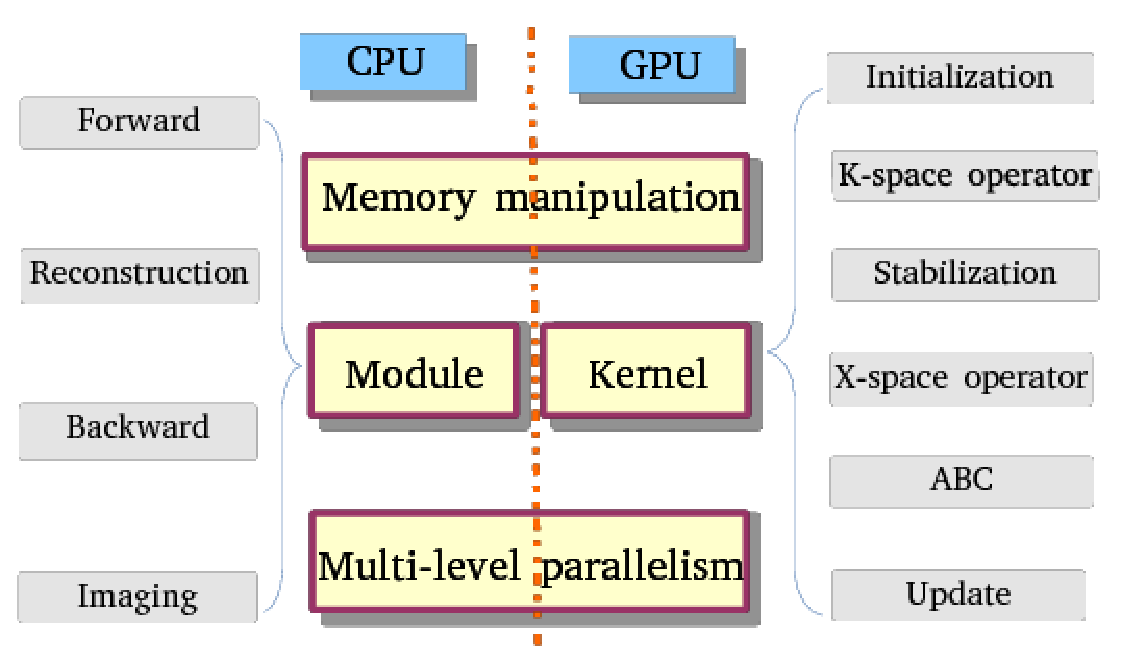
\includegraphics[width=0.8\linewidth]{Fig1.pdf} 
%\caption{The architecture of the cuQ-RTM code package. \label{fig:Fig1}} 
%\end{center} 
%\end{figure}

\plot{Fig1}{width=0.8\linewidth}{The architecture of the cuQ-RTM code package. }



\begin{table}
\begin{center}
\caption{Some important variables allocated on host and device.}
\label{tbl:tab1}
\newcommand{\tabincell}[2]{\begin{tabular}{@{}#1@{}}#2\end{tabular}}
\begin{tabular}{|c|c|c|c|}
\hline {} & Memory type & \tabincell{c}{ Allocation \& Free} & Variables \\
\hline 
\multirow{2}*{Host} & pageable & \tabincell{c}{ \texttt{malloc()} \\ \texttt{free()}} &
 \tabincell{c}{\emph{ricker, vp, Qp, Gamma, t\_cp} \\ \emph{kfilter, kstabilization} \\  \emph{Final\_image\_cor, Final\_image\_cor}} \\
\cline{2-4}
                     & page-locked  & \tabincell{c}{ \texttt{cudaMallocHost()} \\ \texttt{cudaFreeHost()} } & \tabincell{c}{\emph{u0, u1, u2} \\ \emph{seismogram\_obs, seismogram\_rms}  \\  \emph{image\_cor, image\_nor}}  \\
\hline
Device & global & \tabincell{c}{ \texttt{cudaMalloc()} \\ \texttt{cudaFree()} } & \tabincell{c}{\emph{d\_ricker, d\_vp, d\_Gamma, d\_t\_cp, d\_u\_cp} \\ \emph{d\_u0, d\_u1,d\_u2, d\_seimogram\_rms} \\ \emph{d\_image\_cor, d\_image\_nor}  \\  \emph{d\_uk, d\_Lap\_uk, d\_amp\_uk, d\_pha\_uk}  \\ \emph{d\_borders\_up, d\_u2\_final0, d\_u2\_final1} }\\
\hline
\end{tabular} 
\end{center}
\end{table}


\subsection{Kernel}

Kernels, the most basic unit of cu$Q$-RTM to accomplish a series of specific tasks such as variable initialization and applying an absorbing boundary condition (ABC), can further be integrated into a fully functional module.  Different variables are initialized with distinct kernels \texttt{cuda\_kernel\_initialization($\ldots$)},  \texttt{cuda\_kernel\_initialization\_images($\ldots$)}, and \texttt{cuda\_kernel\_initialization\_Finals($\ldots$)} based on their scope in modules.  Wavefield variables are updated by \texttt{cuda\_kernel\_update($\ldots$)}.

In the framework of cu$Q$-RTM, the basic forward and backward modules based on viscoacoustic wave equation with DFLs are efficiently simulated by PSM coupled with the CUFFT library. However, CUFFT library functions can only be executed on the device and called from the host, so we split the customized kernel functions into a k-space component and x-space component. The Fourier transform function \texttt{cufftExecC2C($\ldots$, CUFFT\_FORWARD)} and inverse Fourier transform function \texttt{cufftExecC2C($\ldots$, CUFFT\_INVERSE)} serve as the link between the x-space operator \texttt{cuda\_kernel\_visco\_PSM\_2d\_forward\_x\_space($\ldots$)} and the k-space operator \texttt{cuda\_kernel\_visco\_PSM\_2d\_forward\_k\_space($\ldots$)}. Absorbing boundary conditions for these modeling operators are conducted by the multiple transmitting formula (MTF) \texttt{cuda\_kernel\_MTF\_2nd($\ldots$)} \citep{liao1984transmitting}. 

In the cu$Q$-RTM package, we adopt the CATRC scheme to reconstruct source wavefields, which combines the efficiency of reverse propagation and the stability of checkpointing. Kernel functions \texttt{cuda\_kernel\_checkpoints\_Out($\ldots$)} and \texttt{cuda\_kernel\_checkpoints\_In($\ldots$)} are designed to record and fetch forward wavefields at predefined checkpoints. Furthermore,  wavefields on the outermost layer boundary of simulation domain at each time step are also recorded in global device variables $d\_borders\_up,\ d\_borders\_bottom,\ d\_borders\_left$, and $d\_borders\_right$.  The total memory storage for 2D reconstruction can be estimated as
\begin{equation}
\label{eq:Mem2d}
Storage_{2D}\ [GB] \approx \frac{2(nx+nz) nt + (N_c+2) (nx \times nz)}{1024^3/4},
\end{equation}
and for the 3D case, 
\begin{equation}
\label{eq:Mem3d}
Storage_{3D}\ [GB] \approx \frac{2(nx \times ny + nx \times nz + ny \times nz) nt + (N_c+2) (nx \times ny \times nz)}{1024^3/4},
\end{equation}
where $nx,\ ny,\ nz$ and $nt$ are spatial and temporal grid sizes. Figure \ref{fig:Fig2a_v} shows memory storage against the scale of the model (where we denote size of the simulation as $nx = ny = nz = 0.1 nt = 10 Nc$) for 2D and 3D cases. Figure \ref{fig:Fig2b_v} presents the memory ratio between boundary savings and checkpointing savings for 2D and 3D cases. Such a large amount of memory storage is  unacceptable for the 3D case, so we have to output the boundary savings to the disk and then read the borders by memory copying between host and device memory. 


\multiplot{2}{Fig2a_v,Fig2b_v}{width=0.8\textwidth}{(a) Memory storage and (b) memory ratio of boundary wavefield to checkpointing wavefield (B/C) for both 2D and 3D cases.}


I develop an adaptive stabilization method to deal with numerical instability in $Q$-RTM, which exhibits superior properties of time-variance and $Q$-dependence over conventional low-pass filtering. Both the adaptive stabilization scheme \texttt{cuda\_kernel\_AdaSta($\ldots$)} and low-pass filtering scheme \texttt{cuda\_kernel\_filter2d($\ldots$)} are provided in this package. Users can choose either of these two stabilizing methods to suppress high-frequency noises as they like.

\subsection{Module}

Much as the kernel layer insulates the user from the programming details of a series of specific tasks, the module layer insulates the user from the implementation details of the module of $Q$-RTM, which contains forward extrapolation, wavefield reconstruction, backward extrapolation and imaging. Each of them is made up of several kernel functions and streams. A stream is defined by creating a stream object using \texttt{cudaStreamCreate($\ldots$)} and specifying it as the stream parameter to a sequence of kernel launches and host-device memory copies. Streams are released by calling \texttt{cudaStreamDestroy($\ldots$)}, which waits for all preceding commands in the given stream to complete before destroying the stream and returning control to the host thread. THe forward module \texttt{cuda\_visco\_PSM\_2d\_forward($\ldots$)} in cu$Q$-RTM is designed in a splitting fashion and called by the main function to conduct forward wavefield extrapolation. As wavefield reconstruction, backward extrapolation and imaging are conducted during time-reversal simulation, these three modules can be merged into one module \texttt{cuda\_visco\_PSM\_2d\_backward($\ldots$)}. Both forward and backward modules are presented by brief codes in Appendix A.

\subsection{Multi-level parallelism}

The code package described above is implemented for multiple NVIDIA GPUs using MPI, C, and CUDA in an MLP fashion. The execution is divided into two components. The first is responsible for the coarse-grained parallelization between nodes of the clusters, which is parallelized using MPI. The second performs calculations within each GPU using CUDA. One of the most important issues arising when working with a hybrid MPI/CUDA code is the proper mapping of MPI processes and threads to GPUs and nodes. Thus, we can evenly distribute all shots among every node and every GPU, while being aware of the precise index of each shot during simulation. In the package, we provide two distributing schemes to allow the framework to run on both uniform clusters (i.e., each node with the same number of integrated GPUs) and non-uniform clusters (i.e., a mixture of nodes with the different number and the types of integrated GPUs). Every MPI process (rank) \texttt{MPI\_Comm\_rank(comm,\&myid)} inspects the configuration of the node being executed on, and all GPUs of each node are launched by streaming execution. Algorithms 1 and 2 provide shot distributing schemes to ensure load balancing on each node and device. All threads on host are synchronized by \texttt{MPI\_Barrier(comm)} before migrated images from all shots are reduced by \texttt{MPI\_Allreduce($\ldots$)}, which further guarantees less thread blocking time.

\begin{algorithm}{Algorithm 1: Shot distribution for uniform clusters}{}
     \textbf{Input:} \text{The number of shots} ns, \text{nodes} np, \text{GPUs per node} ng. \\
     \textbf{Output:} \text{Index of each shot}  is. \\
     nsid=ns/(np\times ng)\\
     modsr=ns\%(np\times ng) \\
     prcs=modsr/ng \\
    \begin{IF}{myid<prcs} 
     eachsid=nsid+1;\\
     \text{offset} = myid\times (nsid+1)\times ng;\\
    \ELSE
    eachsid=nsid;\\
    \text{offset}=prcs\times (nsid+1)\times ng+(myid-prcs)\times nsid\times ng;
    \end{IF} \\
    \begin{FOR}{iss\=0\cdots eachsid-1} \\
    \text{offsets} = \text{offset} + iss\times ng; \\ 
    \begin{FOR}{i\=0\cdots ng-1} \\
    is=\text{offsets}+i;  
    \end{FOR}
    \end{FOR}
\end{algorithm}

\begin{algorithm}{Algorithm 2: Shot distribution for non-uniform clusters}{}
     \textbf{Input:} \text{The number of shots} ns, \text{nodes} np, \text{GPUs per node} ng^{(id)}. \\
     \textbf{Output:} \text{Index of each shot}  is. \\
     nsid=ns/\sum_{id=0}^{np-1}{ng^{(id)}}\\
     modsr=ns\%\sum_{id=0}^{np-1}{ng^{(id)}} \\
    \begin{FOR}{j\=1\cdots np-1} \\
    prcs=modsr/\sum_{id=0}^{np-1-j}{ng^{(id)}}; \\ 
    \begin{IF}{prcs>0} 
		break;
    \end{IF} \\
    \end{FOR}
    \begin{IF}{myid<np-j} 
     eachsid=nsid+prcs;\\
     \text{offset} = (nsid+prcs)\times \sum_{id=0}^{myid}{ng^{(id)}};\\
    \ELSE
    eachsid=nsid;\\
    \text{offset}== (nsid+prcs)\times \sum_{id=0}^{np-1-j}{ng^{(id)}}+nsid\times \sum_{id=np-j}^{myid}{ng^{(id)}};
    \end{IF} \\
    \begin{FOR}{iss\=0\cdots eachsid-1} \\
    \text{offsets} = \text{offset} + iss\times ng^{(myid)}; \\ 
    \begin{FOR}{i\=0\cdots ng^{(myid)}-1} \\
    is=\text{offsets}+i; 
    \end{FOR}
    \end{FOR}
\end{algorithm}



\section{Examples}

In this section, we use both synthetic and field examples to demonstrate the superior performance of the presented cu$Q$-RTM package over traditional CPU-based computational models in terms of efficiency, memory storage and stability. All of the following examples are reproducible when the C, CUDA, Matlab and Madagascar platforms \citep{Fomel2013Madagascar} are available. 

\subsection{Viscoacoustic modeling on a layered model}

In the first synthetic example, we perform viscoacoustic modeling on a multi-scale layered model with a single GeForce GTX760 GPU and a single core of Intel Core i5-4460 CPU for speedup comparison. As is shown in Figure \ref{fig:Fig3_v}, the scale of these layered models varies from $128\times 128$ to $2048\times 2048$ grids. We record the mean runtime per time step of viscoacoustic modeling using a single CPU core and a single GPU at each model scale, and their corresponding speedup ratio, which are presented in Table \ref{tbl:tab2}. CPU-based simulation is compiled by GNU C++ compiler (g++ 4.8.4) with FFTW 3.3.2. GPU-based simulation is compiled by CUDA C with the CUFFT library API. Figure \ref{fig:Fig4_v} shows the mean runtime per time step and the corresponding speedup ratio against model scale. It indicates that the presented cu$Q$-RTM package running on a single GPU card can nearly be 50-80 times faster than the conventional CPU implementation with a single CPU core. Furthermore, simulation on a larger model scale tends to achieve a greater speedup ratio.


\plot{Fig3_v}{width=0.6\linewidth}{Velocity  models for multi-scale layered model.}

\begin{table}
\caption{The mean runtime per time step of viscoacoustic modeling using  a single GTX760 GPU relative to a four-core Intel Core i5-4460 CPU and the corresponding speedup ratio against model scale.}
\label{tbl:tab2}
\begin{center}
\begin{tabular}{|c|c|c|c|c|c|}
\hline Model Scale (grids) & 128 $\times$ 128  & 256 $\times$ 256 & 512 $\times$ 512 & 1024 $\times$ 1024 & 2048 $\times$ 2048\\
\hline CPU Runtime (ms) & 9.7170 & 43.5925 & 101.3938 & 359.0682 & 1855.8382\\
\hline GPU Runtime (ms) & 0.1839 & 0.8195 & 1.8262 & 6.3267 & 22.3263\\
\hline Speedup Ratio & 52.8385 & 53.1940 & 55.5217 & 56.7544 & 83.1234\\
\hline
\end{tabular} 
\end{center}
\end{table}


\plot{Fig4_v}{width=0.6\linewidth}{The mean runtime per time step of viscoacoustic modeling using a single GTX760 GPU relative to a four-core Intel Core i5-4460 CPU and the corresponding speedup ratio against model scale.}

\subsection{$Q$-RTM on Marmousi model}

The second synthetic example presented here is CUDA-based $Q$-RTM for the Marmousi model. Figures \ref{fig:vp} and \ref{fig:qp} show its velocity and $Q$ models, which contains a high-attenuation zone with a low $Q$ value. The model has 234 nodes with a sampling interval of $dz=10$ m in depth and 663 nodes with a sampling interval of $dx=10$ m  in the horizontal direction. In the observation system, 60 sources are distributed laterally with a shot interval $ds=100$ m, and each shot has 301 double-sided receivers with a maximum offset of 1500 m.  The point source is a Ricker wavelet with a dominant frequency $f_d=20$ Hz. The synthetic seismic data are modeled by the PSM with time interval $dt=0.001$ s, and the records last 2 s.  

Figure \ref{fig:img0,img1,img2,img3} shows the migrated image using conventional RTM from acoustic data (Figure \ref{fig:img0}) and viscoacoustic data without compensation (Figure \ref{fig:img1}), and $Q$-RTM from viscoacoustic data (Figures \ref{fig:img2} and \ref{fig:img3}), respectively. The acoustic imaging result shown in Figure \ref{fig:img0} serves as a reference for comparison. Due to the presence of a high-attenuation zone,  the imaging result of the structure beneath high-attenuation zone shown in the blue frame in Figure \ref{fig:img1} exhibits attenuated amplitudes and blurred structures. The attenuation also severely affects the migrated image of the anticlinal structure, shown in the green frame in Figure \ref{fig:img1} below the unconformity. Figures \ref{fig:img2} and \ref{fig:img3} show compensated images from $Q$-RTM using conventional low-pass filtering and the proposed adaptive stabilization scheme. The compensated images exhibit a clear anticlinal structure and recovered amplitudes compared with the non-compensated image. For another comparison, Figure \ref{fig:Fig7a_v,Fig7b_v,Fig7c_v} shows migrated seismic traces, which are selected arbitrarily at three distances of 1500 m, 3600 m and 5200 m from the imaging results shown in Figure \ref{fig:img0,img1,img2,img3}. From these traces, one find that the compensated traces match well with the reference traces. It indicates that the developed cu$Q$-RTM package is capable of improving imaging quality. 

The strong scaling plot shows how the execution time decreases with an increasing number of computing resources. During large-scale imaging, the proportion of computational time  spent to simulate wave propagation mandates that the solver must be efficient and scale well. In this regard, 60 shots of $Q$-RTM are evenly distributed among every GPU card with the number of GPUs (Tesla K10) varying from one to six. We record scheduling runtime and computational runtime during every test and present them in Table \ref{tbl:tab3}. Figure \ref{fig:Fig8_v} shows the results of a strong scaling test of cu$Q$-RTM on the Marmousi model. It demonstrates that very close to ideal efficiency can be achieved with a balanced load on each GPU. Thus, the code package exhibits excellent scalability and can be run with almost ideal code performance, in part because communications are almost entirely overlapped with calculations. 

\inputdir{marm}
\multiplot{2}{vp,qp}{width=0.6\linewidth}{(a) Velocity and (b) $Q$ of the Marmousi model.}

\multiplot{4}{img0,img1,img2,img3}{width=0.45\linewidth}{Migrated images of the Marmousi model using (a) conventional RTM from acoustic data, (b) conventional RTM from viscoacoustic media without compensation, (c) $Q$-RTM using low-pass filtering and (d) $Q$-RTM using adaptive stabilization scheme.}

\inputdir{./}

%\begin{figure}
%\begin{center} 
%\subfigure[]{ 
%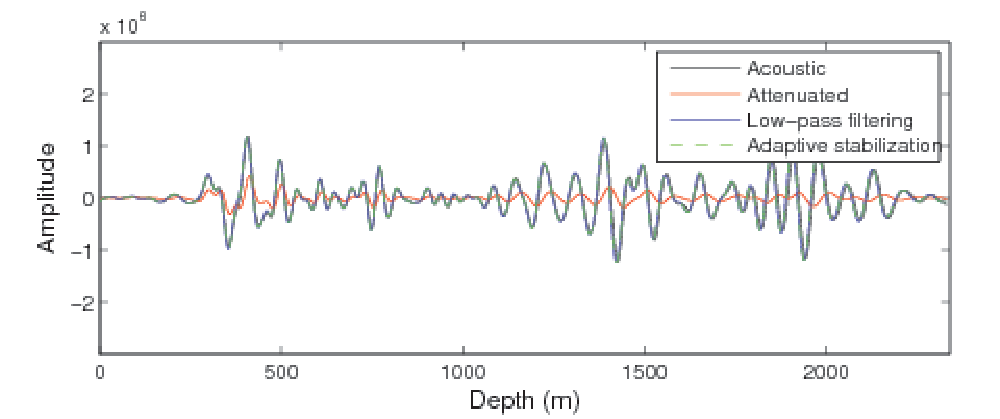
\includegraphics[width=0.6\linewidth]{Fig7a_v.pdf} 
%}
%\subfigure[]{ 
%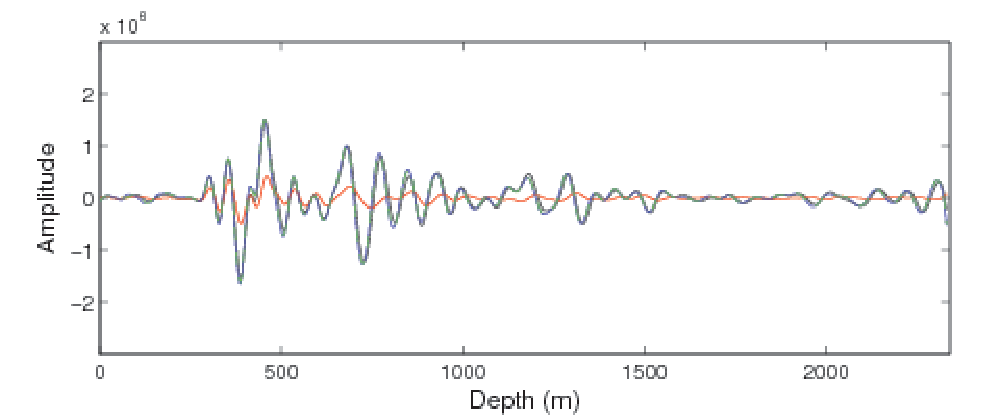
\includegraphics[width=0.6\linewidth]{Fig7b_v.pdf} 
%}
%\subfigure[]{ 
%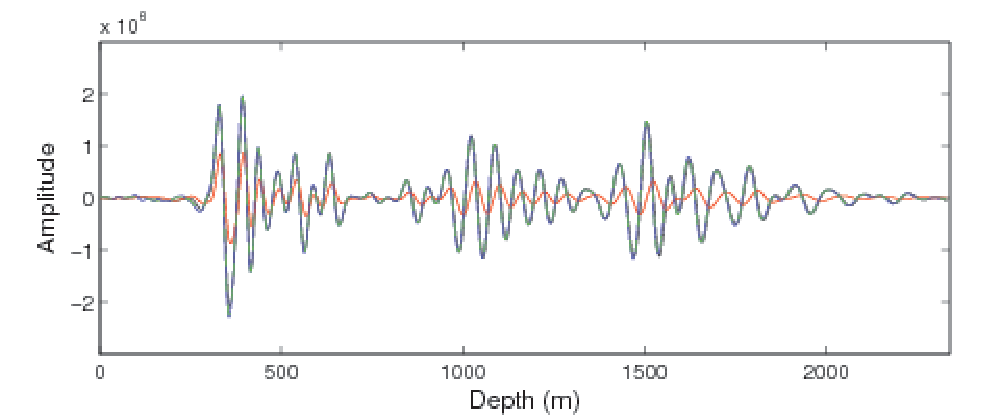
\includegraphics[width=0.6\linewidth]{Fig7c_v.pdf} 
%}
%\caption{Migrated seismic traces selected at three distances of (a) 1500 m, (b) 3600 m and (c) 5200 m from migration results shown in Figure \ref{fig:img0,img1,img2,img3}.  \label{fig:Fig7a_v,Fig7b_v,Fig7c_v}}
%\end{center} 
%\end{figure}

\multiplot{3}{Fig7a_v,Fig7b_v,Fig7c_v}{width=0.45\linewidth}{Migrated seismic traces selected at three distances of (a) 1500 m, (b) 3600 m and (c) 5200 m from migration results shown in Figure \ref{fig:img0,img1,img2,img3}.}



\begin{table}
\caption{runtime of cu$Q$-RTM using multiple Tesla K10 GPUs and the corresponding speedup ratio against the number of GPUs. The model has 234 nodes with in depth and 663 nodes in the horizontal direction.}
\label{tbl:tab3}
\begin{center}
\begin{tabular}{|c|c|c|c|c|c|c|}
\hline The number of GPUs & 1  & 2 & 3 & 4 & 5 & 6\\
\hline Manipulational Runtime (s) & 7.62 & 10.07 & 10.52 & 11.02 & 11.41 & 11.92\\
\hline Computational Runtime (s) & 2639.29 & 1329.40 & 889.82 & 672.78 & 539.21 & 449.97\\
\hline Total Runtime (s) & 2646.91 & 1339.50 & 900.34 & 683.80 & 550.62 & 461.89\\
\hline Speedup Ratio & 1.0000 & 1.9761 & 2.9399 & 3.8709 & 4.8071 & 5.7306\\
\hline
\end{tabular}
\end{center}
\end{table}


%\begin{figure}
%\begin{center} 
%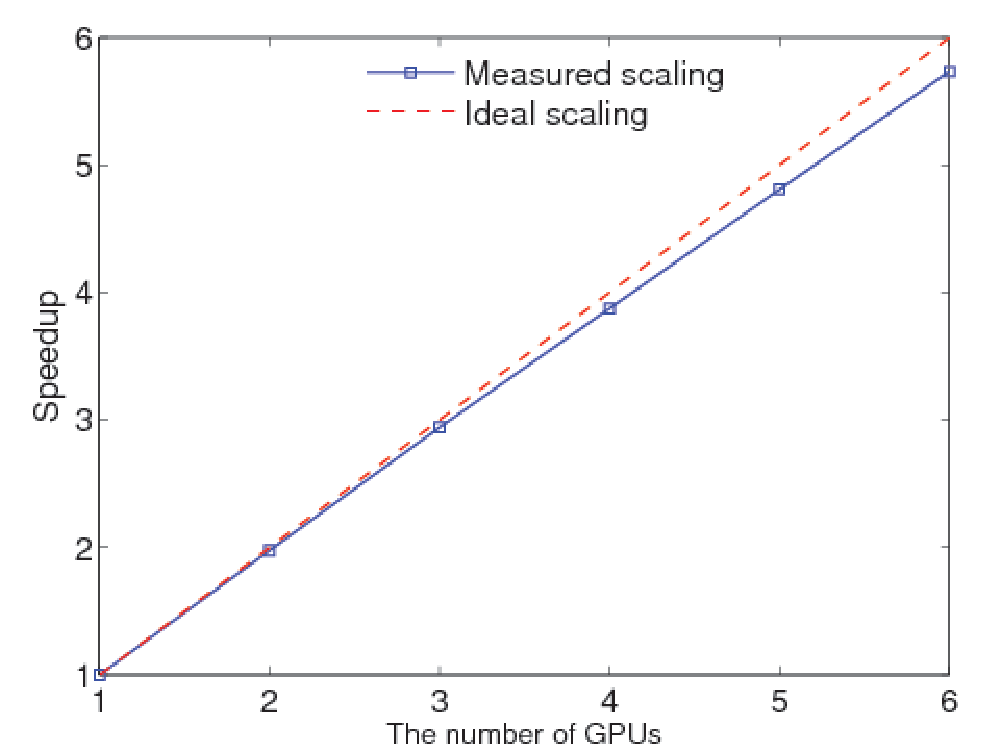
\includegraphics[width=0.6\linewidth]{Fig8_v.pdf} 
%\caption{Strong scaling for cu$Q$-RTM on the Marmousi model using multiple Tesla K10 GPUs. Speedup ratios are plotted against the number of GPUs. The model has 234 nodes with in depth and 663 nodes in the horizontal direction. \label{fig:Fig8_v}}
%\end{center} 
%\end{figure}


\plot{Fig8_v}{width=0.6\linewidth}{Strong scaling for cu$Q$-RTM on the Marmousi model using multiple Tesla K10 GPUs. Speedup ratios are plotted against the number of GPUs. The model has 234 nodes with in depth and 663 nodes in the horizontal direction. }

\subsection{$Q$-RTM on field data}

The field data example shown in Figures \ref{fig:Fig9a_v,Fig9b_v}-\ref{fig:Fig11a_v,Fig11b_v} aims to further verify the feasibility and applicability of the proposed package. Velocity and $Q$ models are presented in Figure \ref{fig:Fig9a_v,Fig9b_v}, which were obtained by migration velocity analysis \citep{sava2008numeric} and $Q$ tomography \citep{shen2015image}. The size of the model is 8.0 km $\times$ 15.6 km with the spatial interval $dx = dz = 10$ m. There are 77 shots horizontally distributed on the surface of the model. We perform $nt = 10000$ time steps for each shot with the temporal interval $dt = 0.0005$ s. In order to eliminate the diffraction artifacts from long offset, we set the stacking aperture of 2.0 km around the shot. Figure \ref{fig:Fig10a_v,Fig10b_v} shows the migrated image using conventional RTM without compensation (Figure \ref{fig:Fig10a_v}) and $Q$-RTM from real data (Figure \ref{fig:Fig10b_v}), respectively. For a clearer comparison, we display the zoomed in seismic images in Figure \ref{fig:Fig11a_v,Fig11b_v} corresponding to the marked area from Figure \ref{fig:Fig10a_v,Fig10b_v}. From Figures \ref{fig:Fig10a_v} and \ref{fig:Fig10b_v}, one can conclude that the $Q$-compensated image using the proposed package exhibits sharper reflections and more balanced amplitude. 


\multiplot{2}{Fig9a_v,Fig9b_v}{width=0.45\linewidth}{(a) Velocity and (b) $Q$ models for field data.}

\multiplot{2}{Fig10a_v,Fig10b_v}{width=0.45\linewidth}{Migrated images of the field data using (a) conventional RTM from viscoacoustic media without compensation, (b) $Q$-RTM.}

\multiplot{2}{Fig11a_v,Fig11b_v}{width=0.45\linewidth}{Zoom view of the images shown in the boxs in (a) Figure \ref{fig:Fig10a_v} and (b) Figure \ref{fig:Fig10b_v}.}



\section{Discussion}

An open-source code package cu$Q$-RTM presented in this chapter is designed for efficient and stable viscoacoustic imaging in attenuating media. The package utilizes streamed CUFFT, CATRC scheme and adaptive stabilization to pertinently tackle some well known problems in viscoacoustic imaging such as intensive computations, large storage requirements and frequent disk I/O, and instability. Each of these issues has been discussed in the literature, notably an efficient implementation of 3D FFTs across multiple-GPU systems \citep{nandapalan2012implementation, czechowski2012communication}, memory-saving reconstruction schemes \citep{Anderson2012Time, yang2016wavefield, wang2017wavefield}, and stabilized compensation strategies \citep{Zhu2014Q, sun2015stable, wang2017regularized}. The proposed package aims at utilizing a set of the state-of-art strategies to achieve an efficient, storage-saving and stable $Q$-RTM. Here we discuss the superior performance of the CATRC scheme and adaptive stabilization over conventional methods. Unlike conventional effective boundary-saving strategy using finite-differences (FD) ($2Lc+1$ grid points FD stencil), which requires $Lc$ layers of boundary wavefields at each time step, the proposed CATRC scheme stores the outermost layers of boundary wavefields at each time step plus states at the checkpoints and the last two time steps to the reconstructed source wavefield for performing crosscorrelating imaging condition, without much loss of precision. Figure \ref{fig:Fig12a_v,Fig12b_v,Fig12c_v,Fig12d_v,Fig12e_v,Fig12f_v} shows source snapshots, reconstructed snapshots and their differences from the Marmousi model at two propagation times. It demonstrates that the reconstructed wavefields from CATRC are accurate enough for $Q$-RTM. 

\multiplot{6}{Fig12a_v,Fig12b_v,Fig12c_v,Fig12d_v,Fig12e_v,Fig12f_v}{width=0.45\linewidth}{Forward snapshots, reconstructed snapshots and their differences from Marmousi model (see Figure \ref{fig:vp,qp}) at two propagation times: (a)-(c) $t=0.82$ s and (d)-(f) $t=1.22$ s.}


%\begin{figure}
%\begin{center} 
%\subfigure[]{ 
%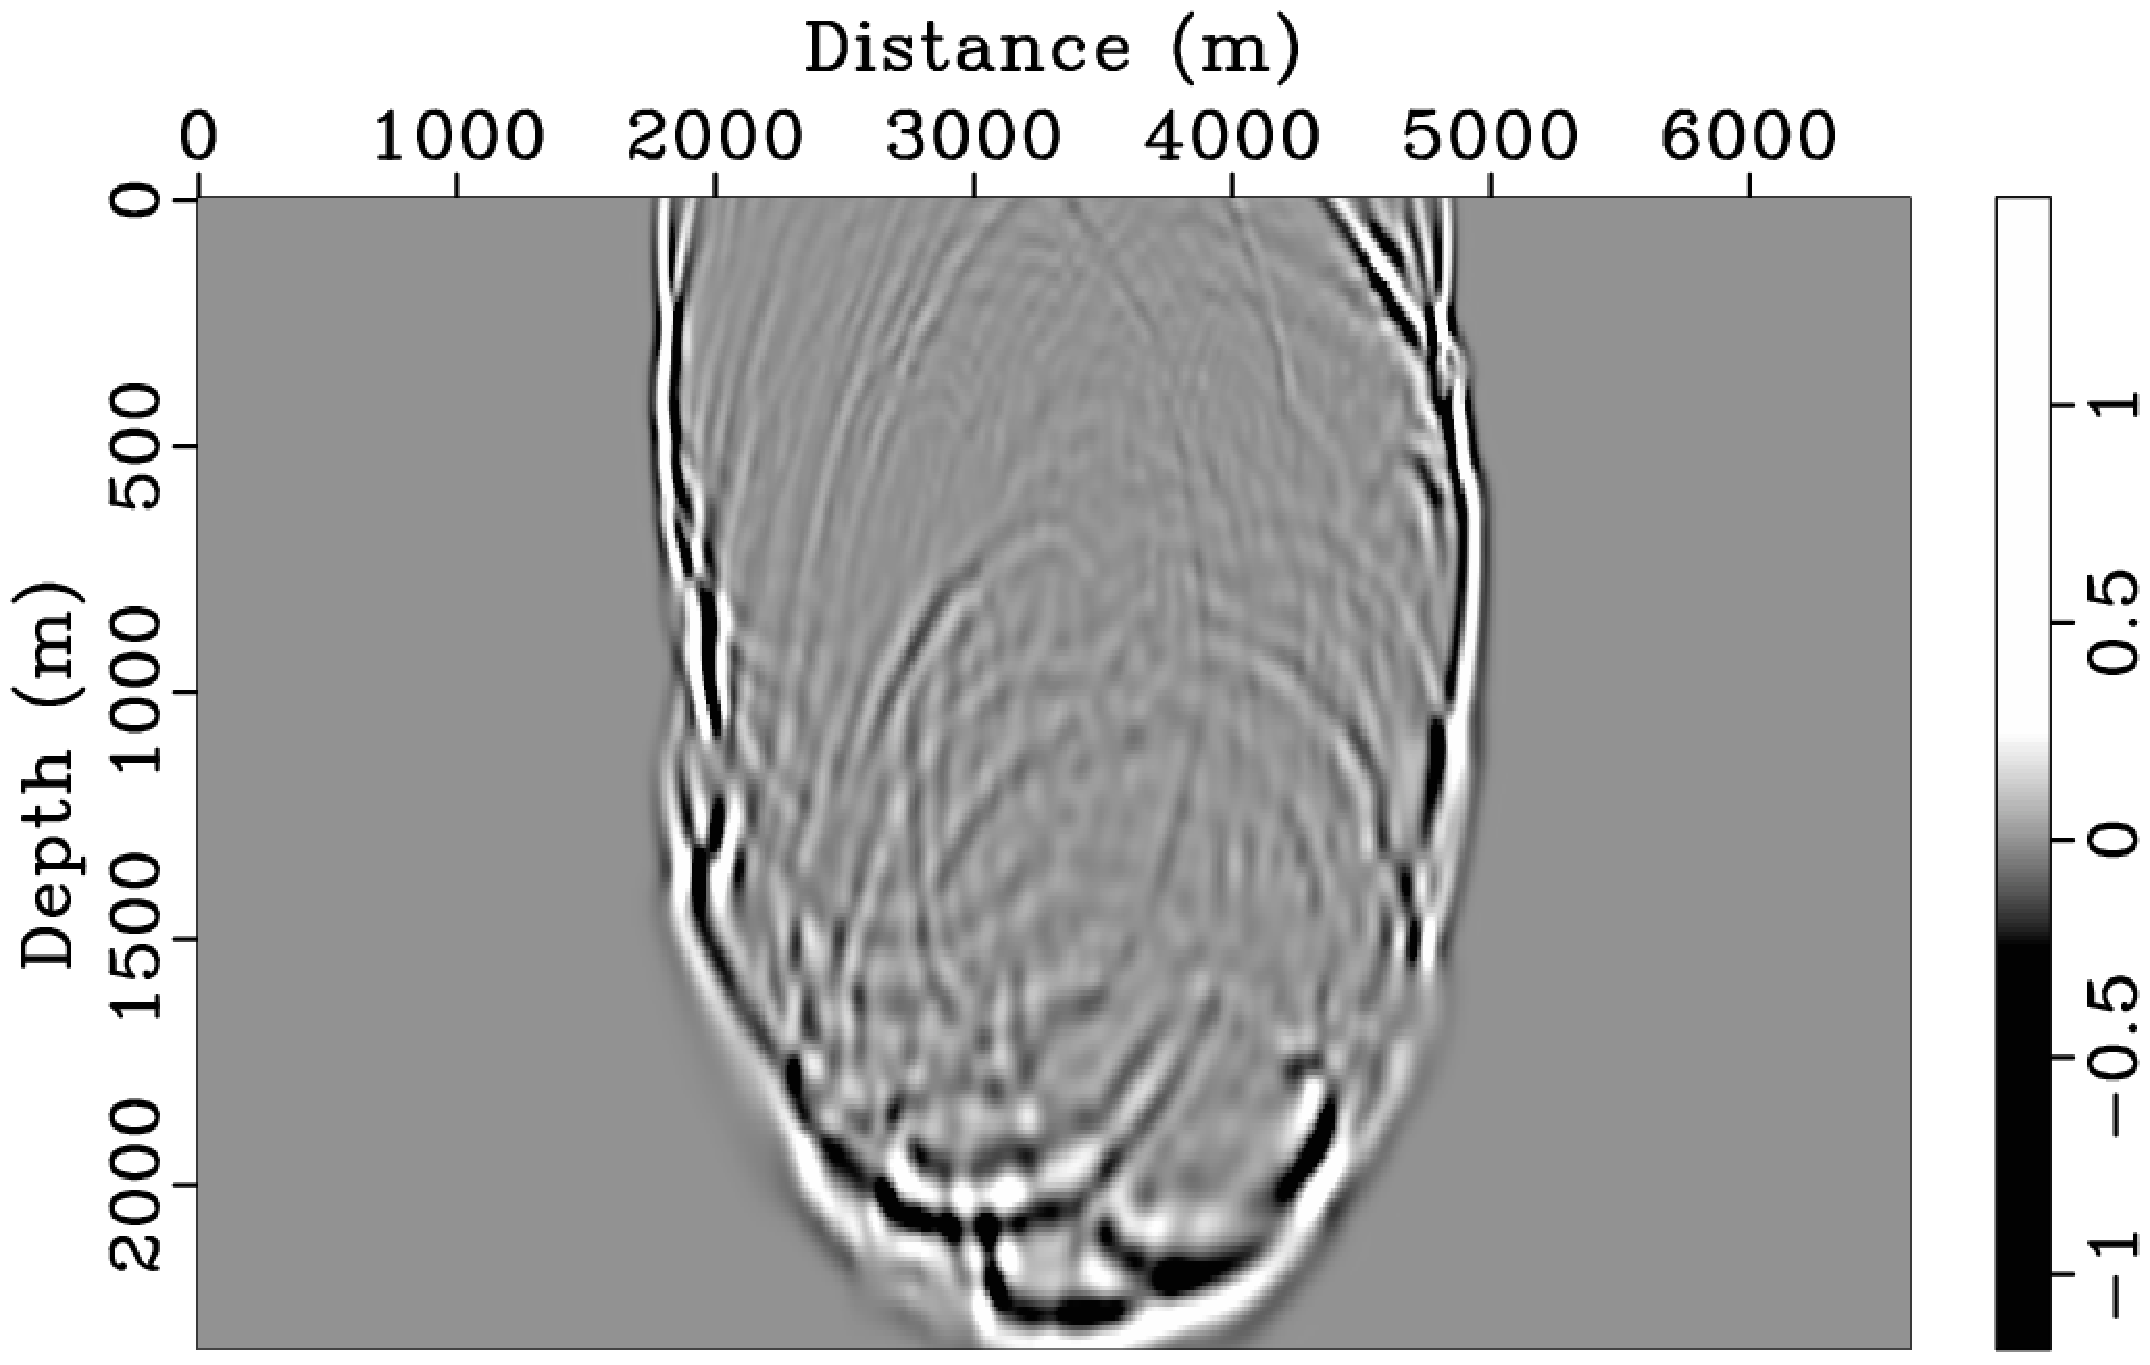
\includegraphics[width=0.3\linewidth]{Fig12a_v.pdf} 
%}
%\subfigure[]{ 
%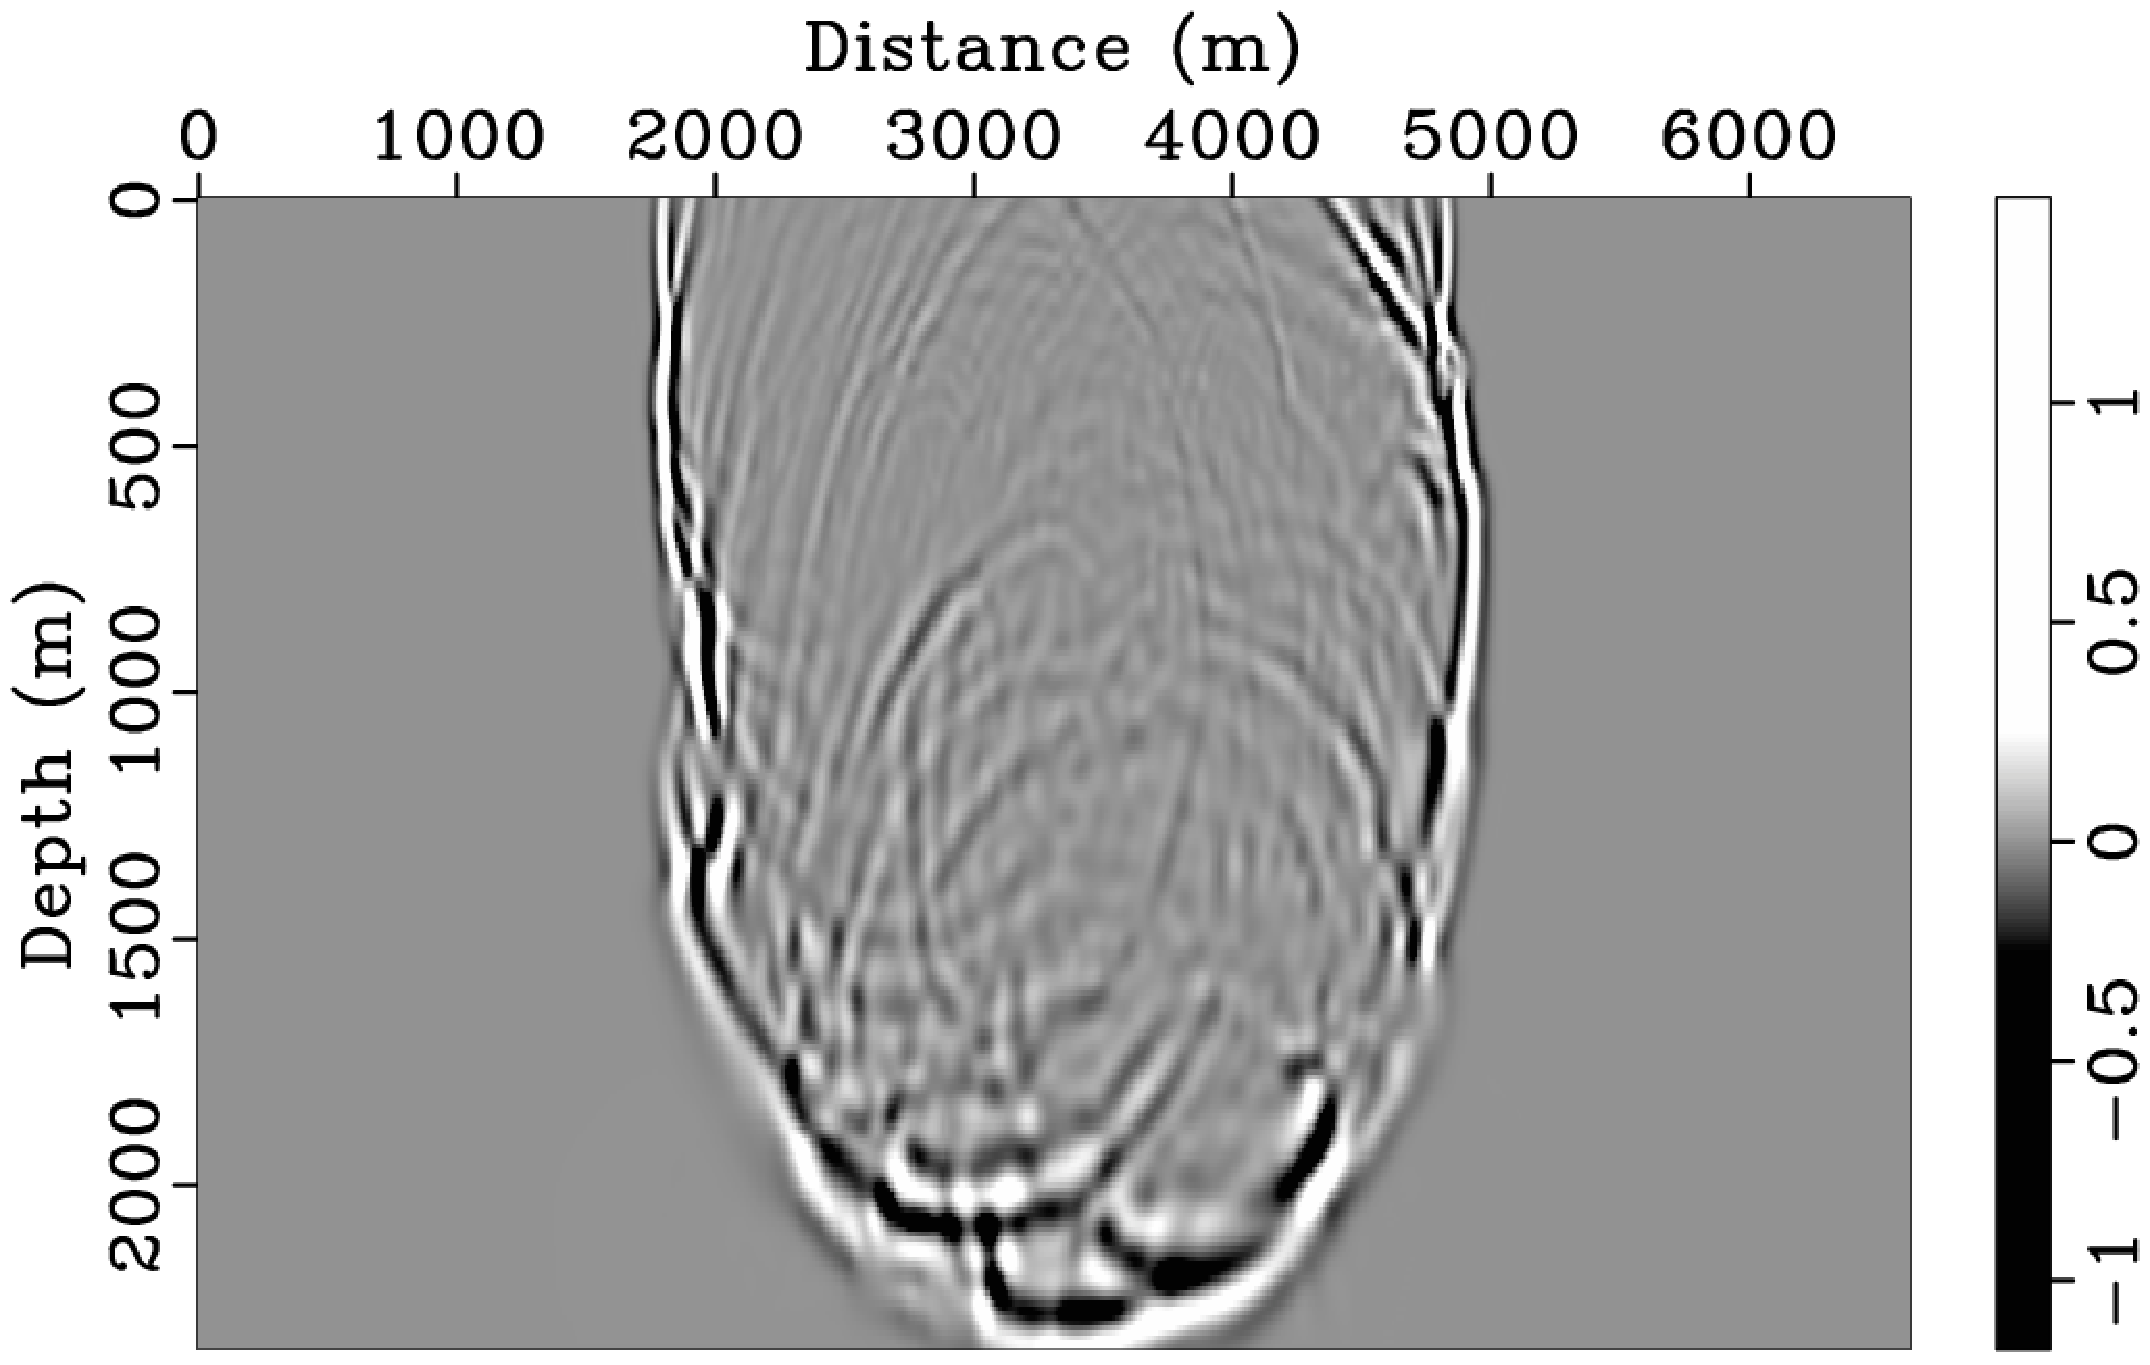
\includegraphics[width=0.3\linewidth]{Fig12b_v.pdf} 
%}
%\subfigure[]{ 
%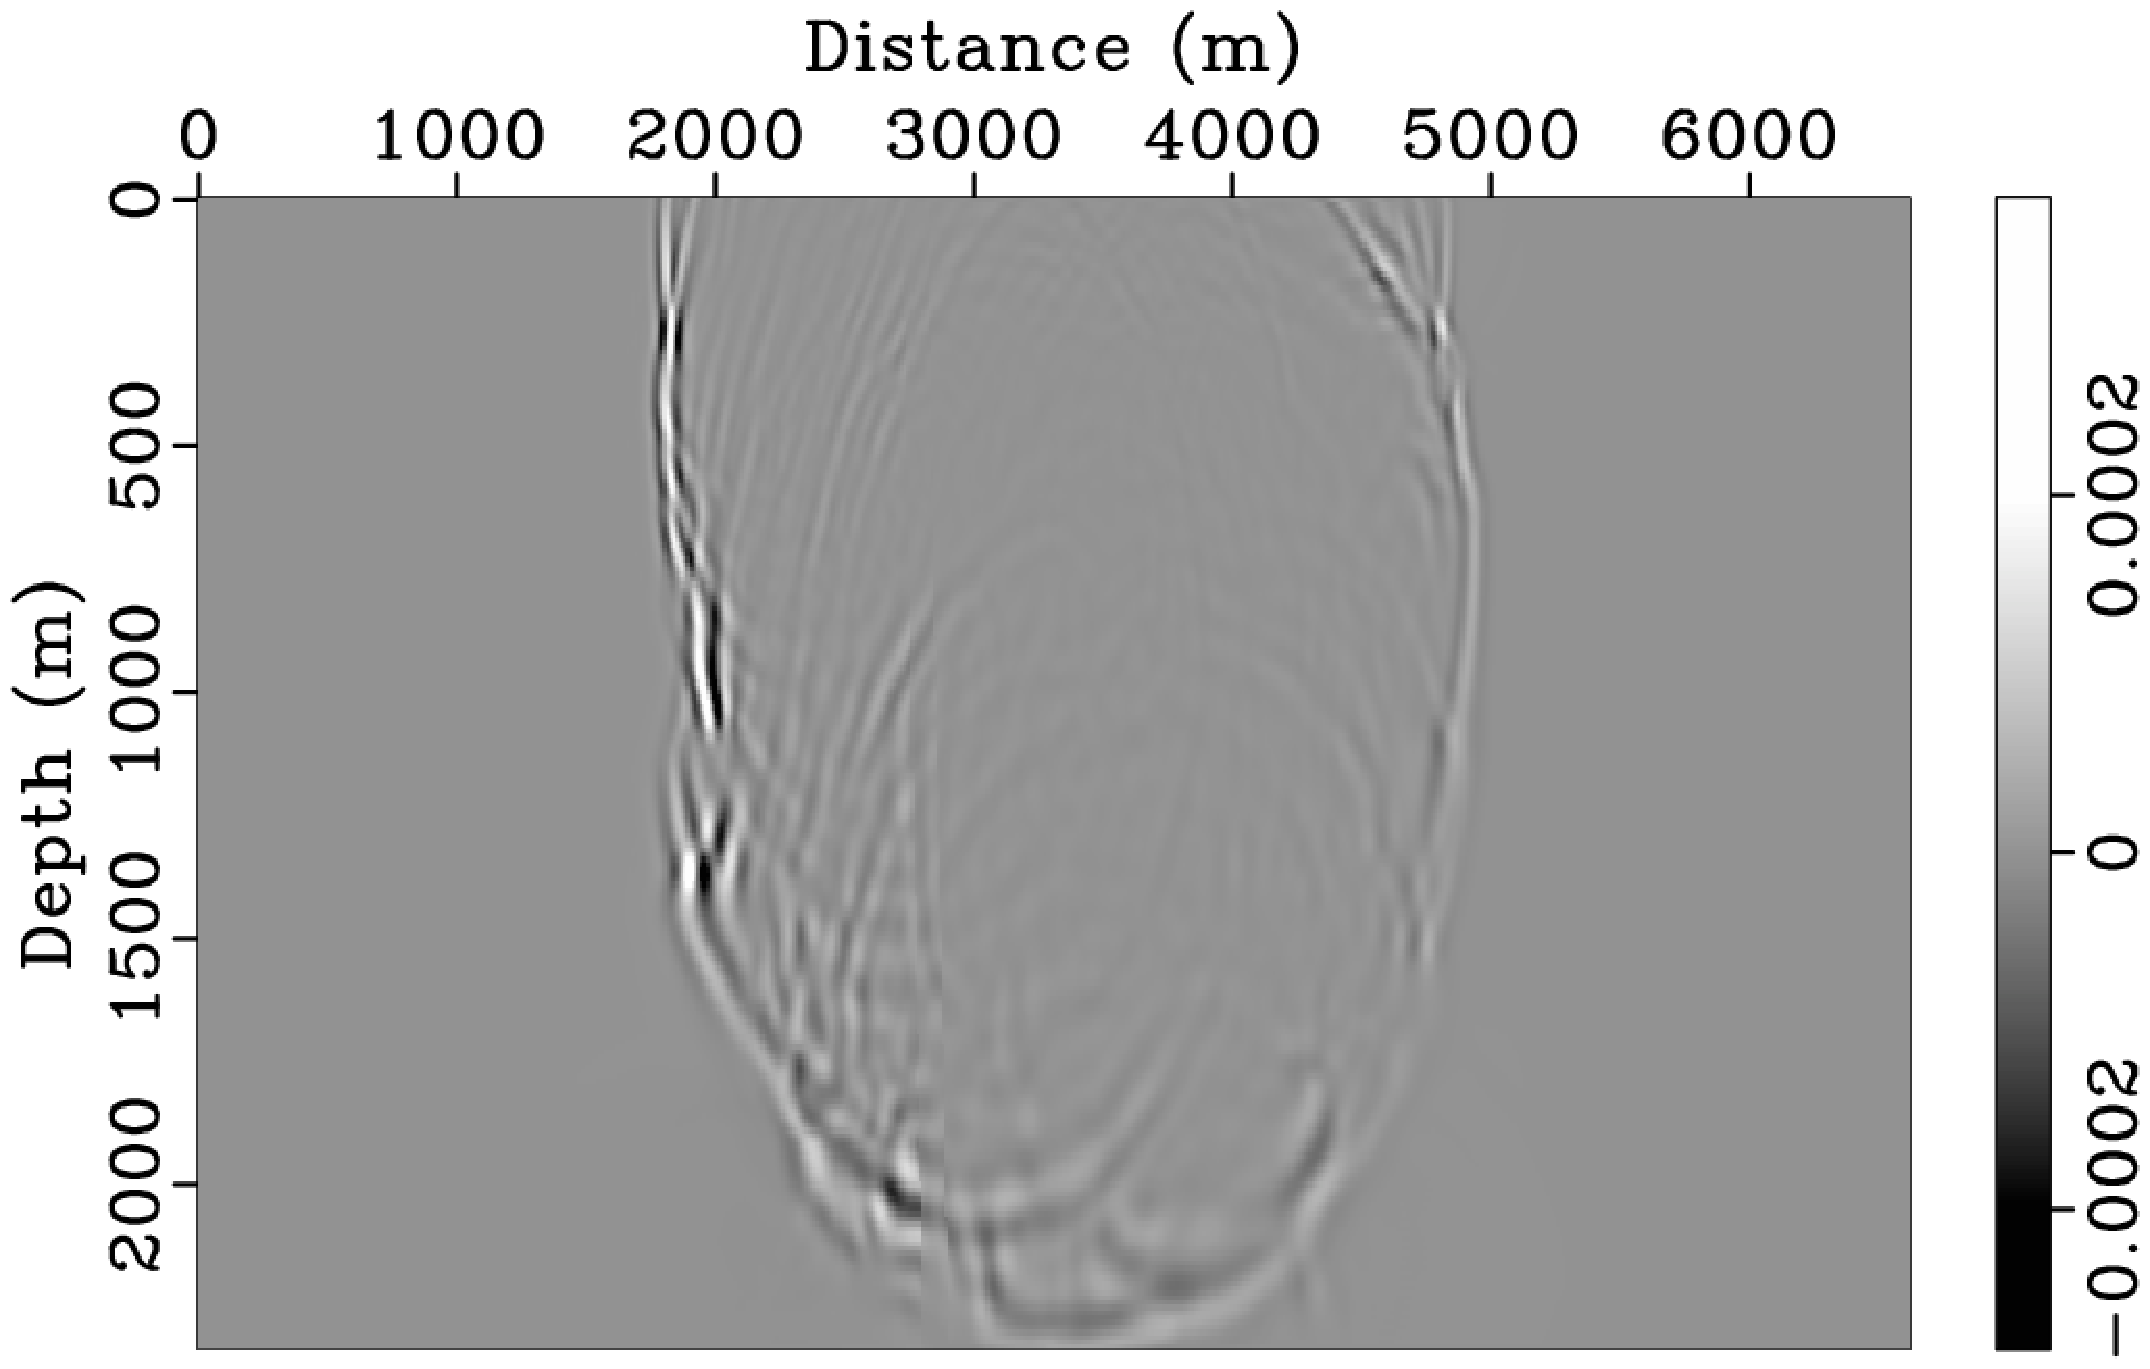
\includegraphics[width=0.3\linewidth]{Fig12c_v.pdf} 
%}
%\subfigure[]{ 
%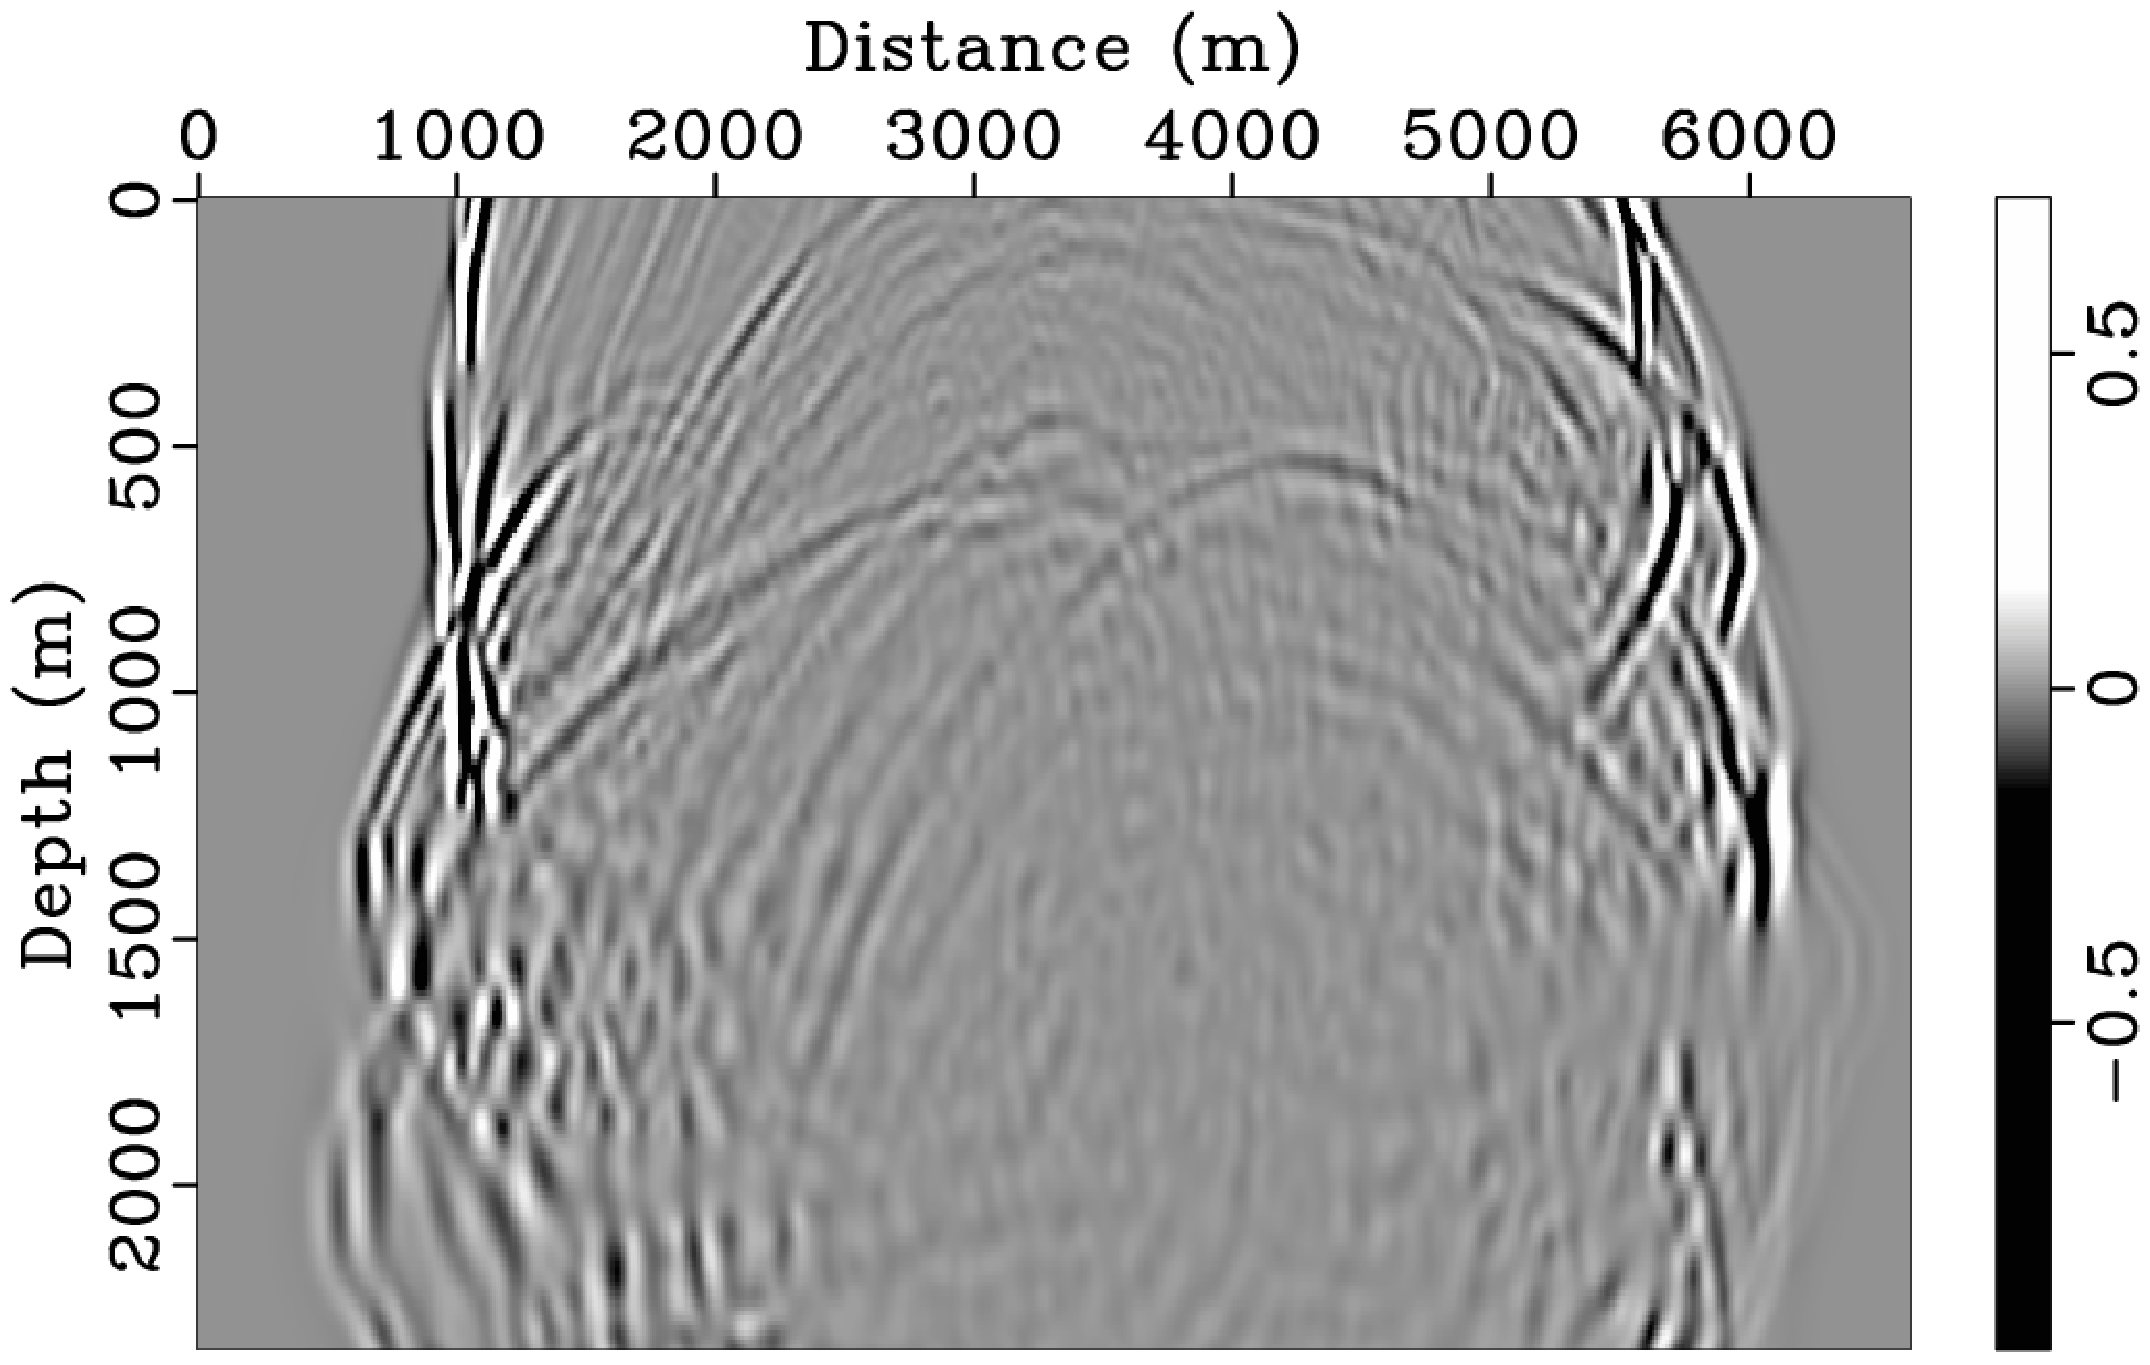
\includegraphics[width=0.3\linewidth]{Fig12d_v.pdf} 
%}
%\subfigure[]{ 
%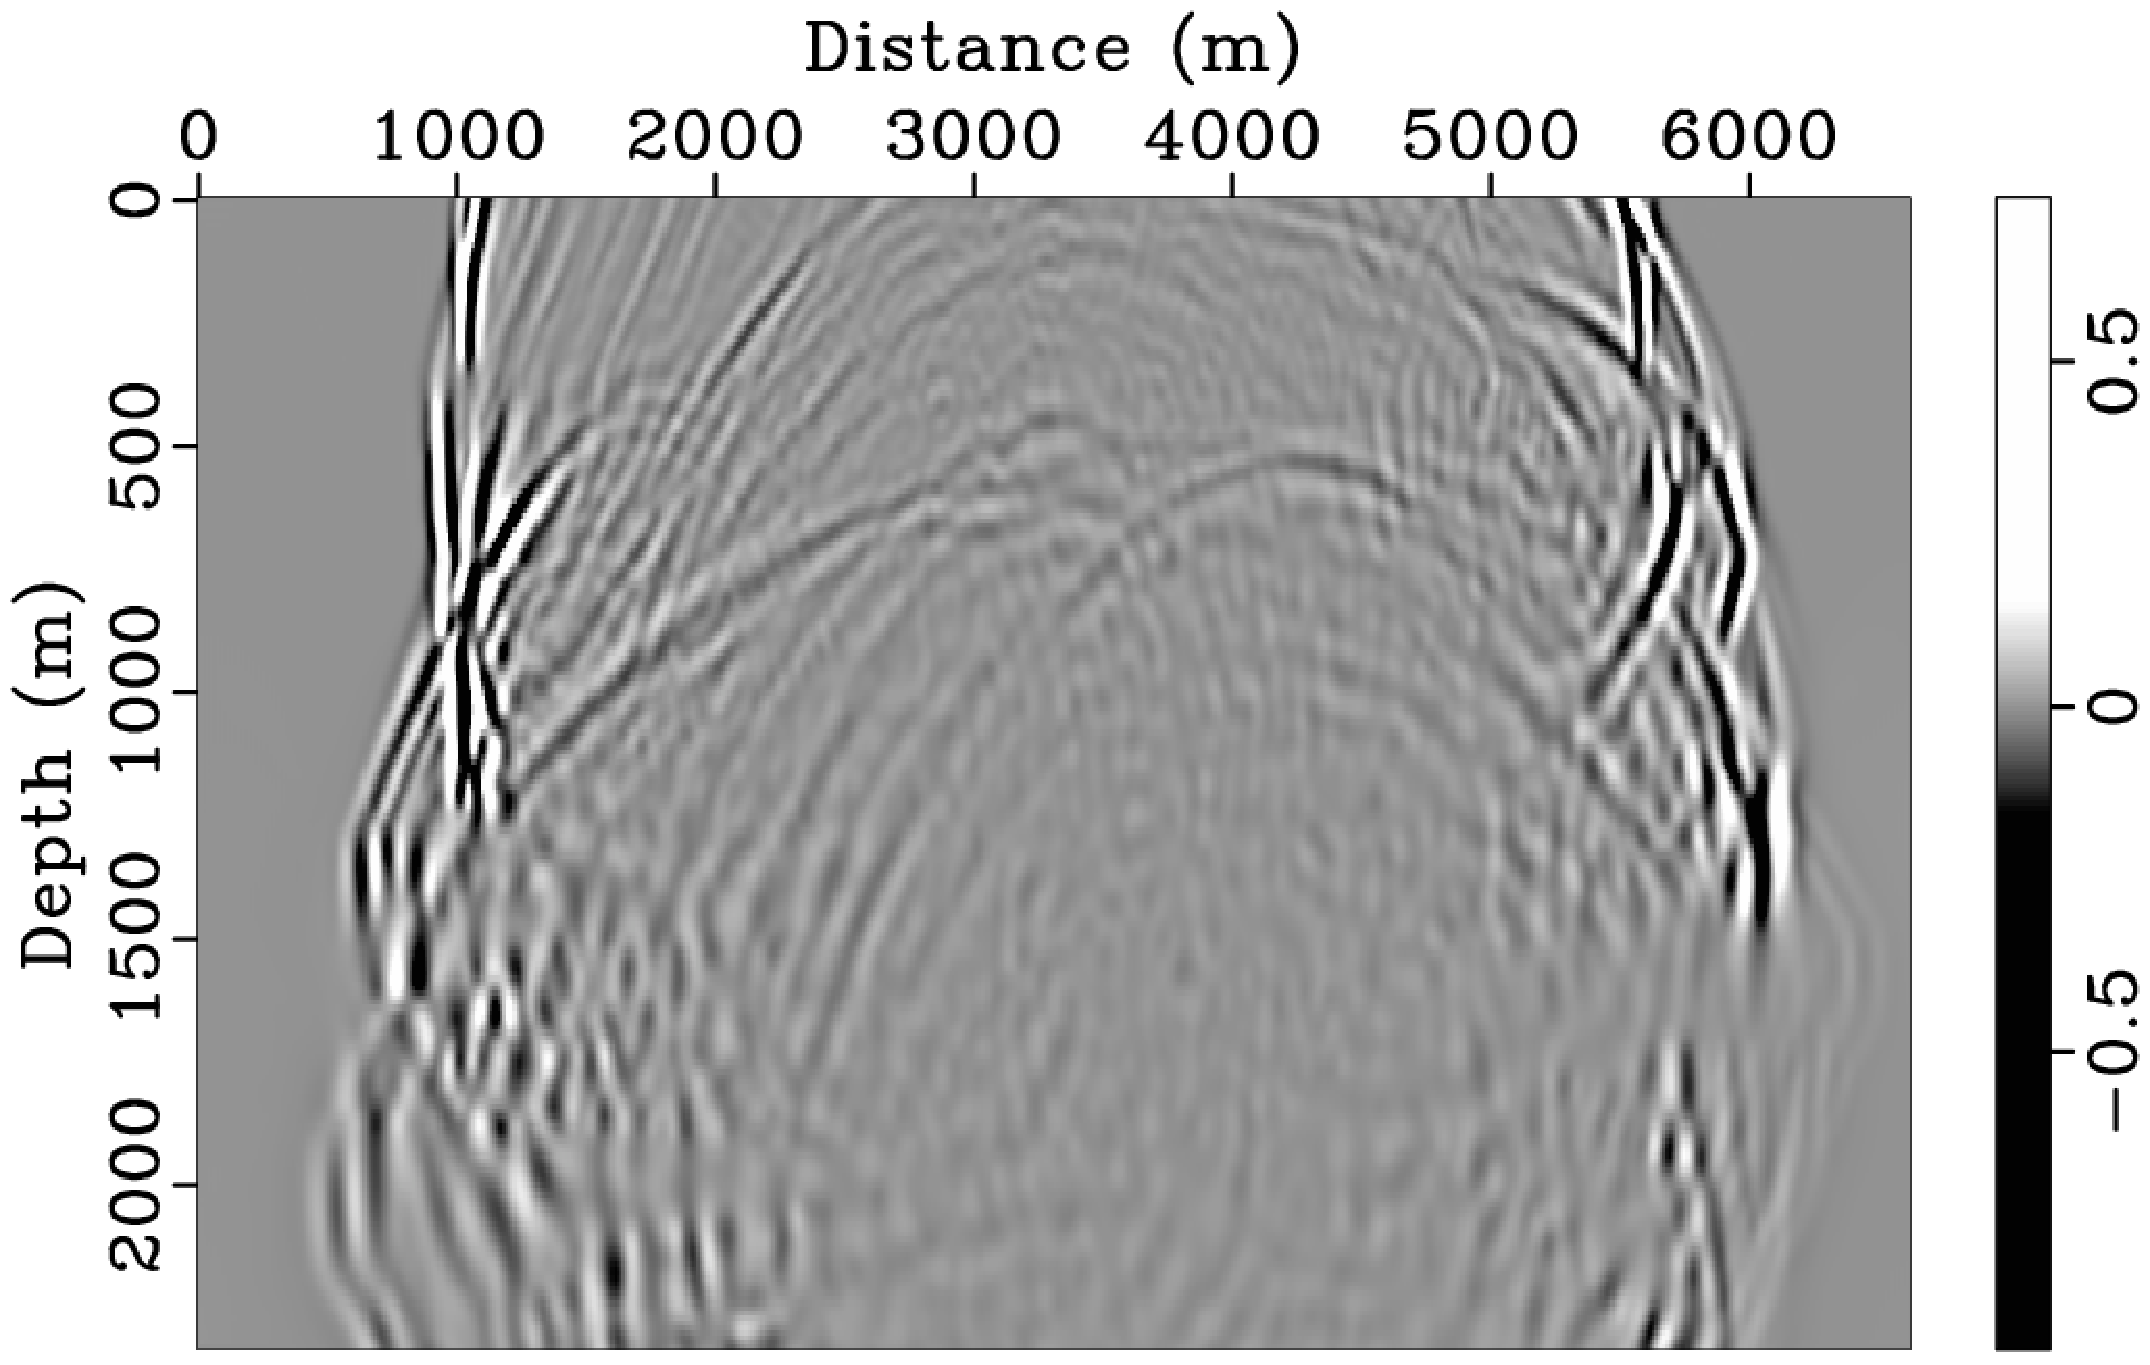
\includegraphics[width=0.3\linewidth]{Fig12e_v.pdf} 
%}
%\subfigure[]{ 
%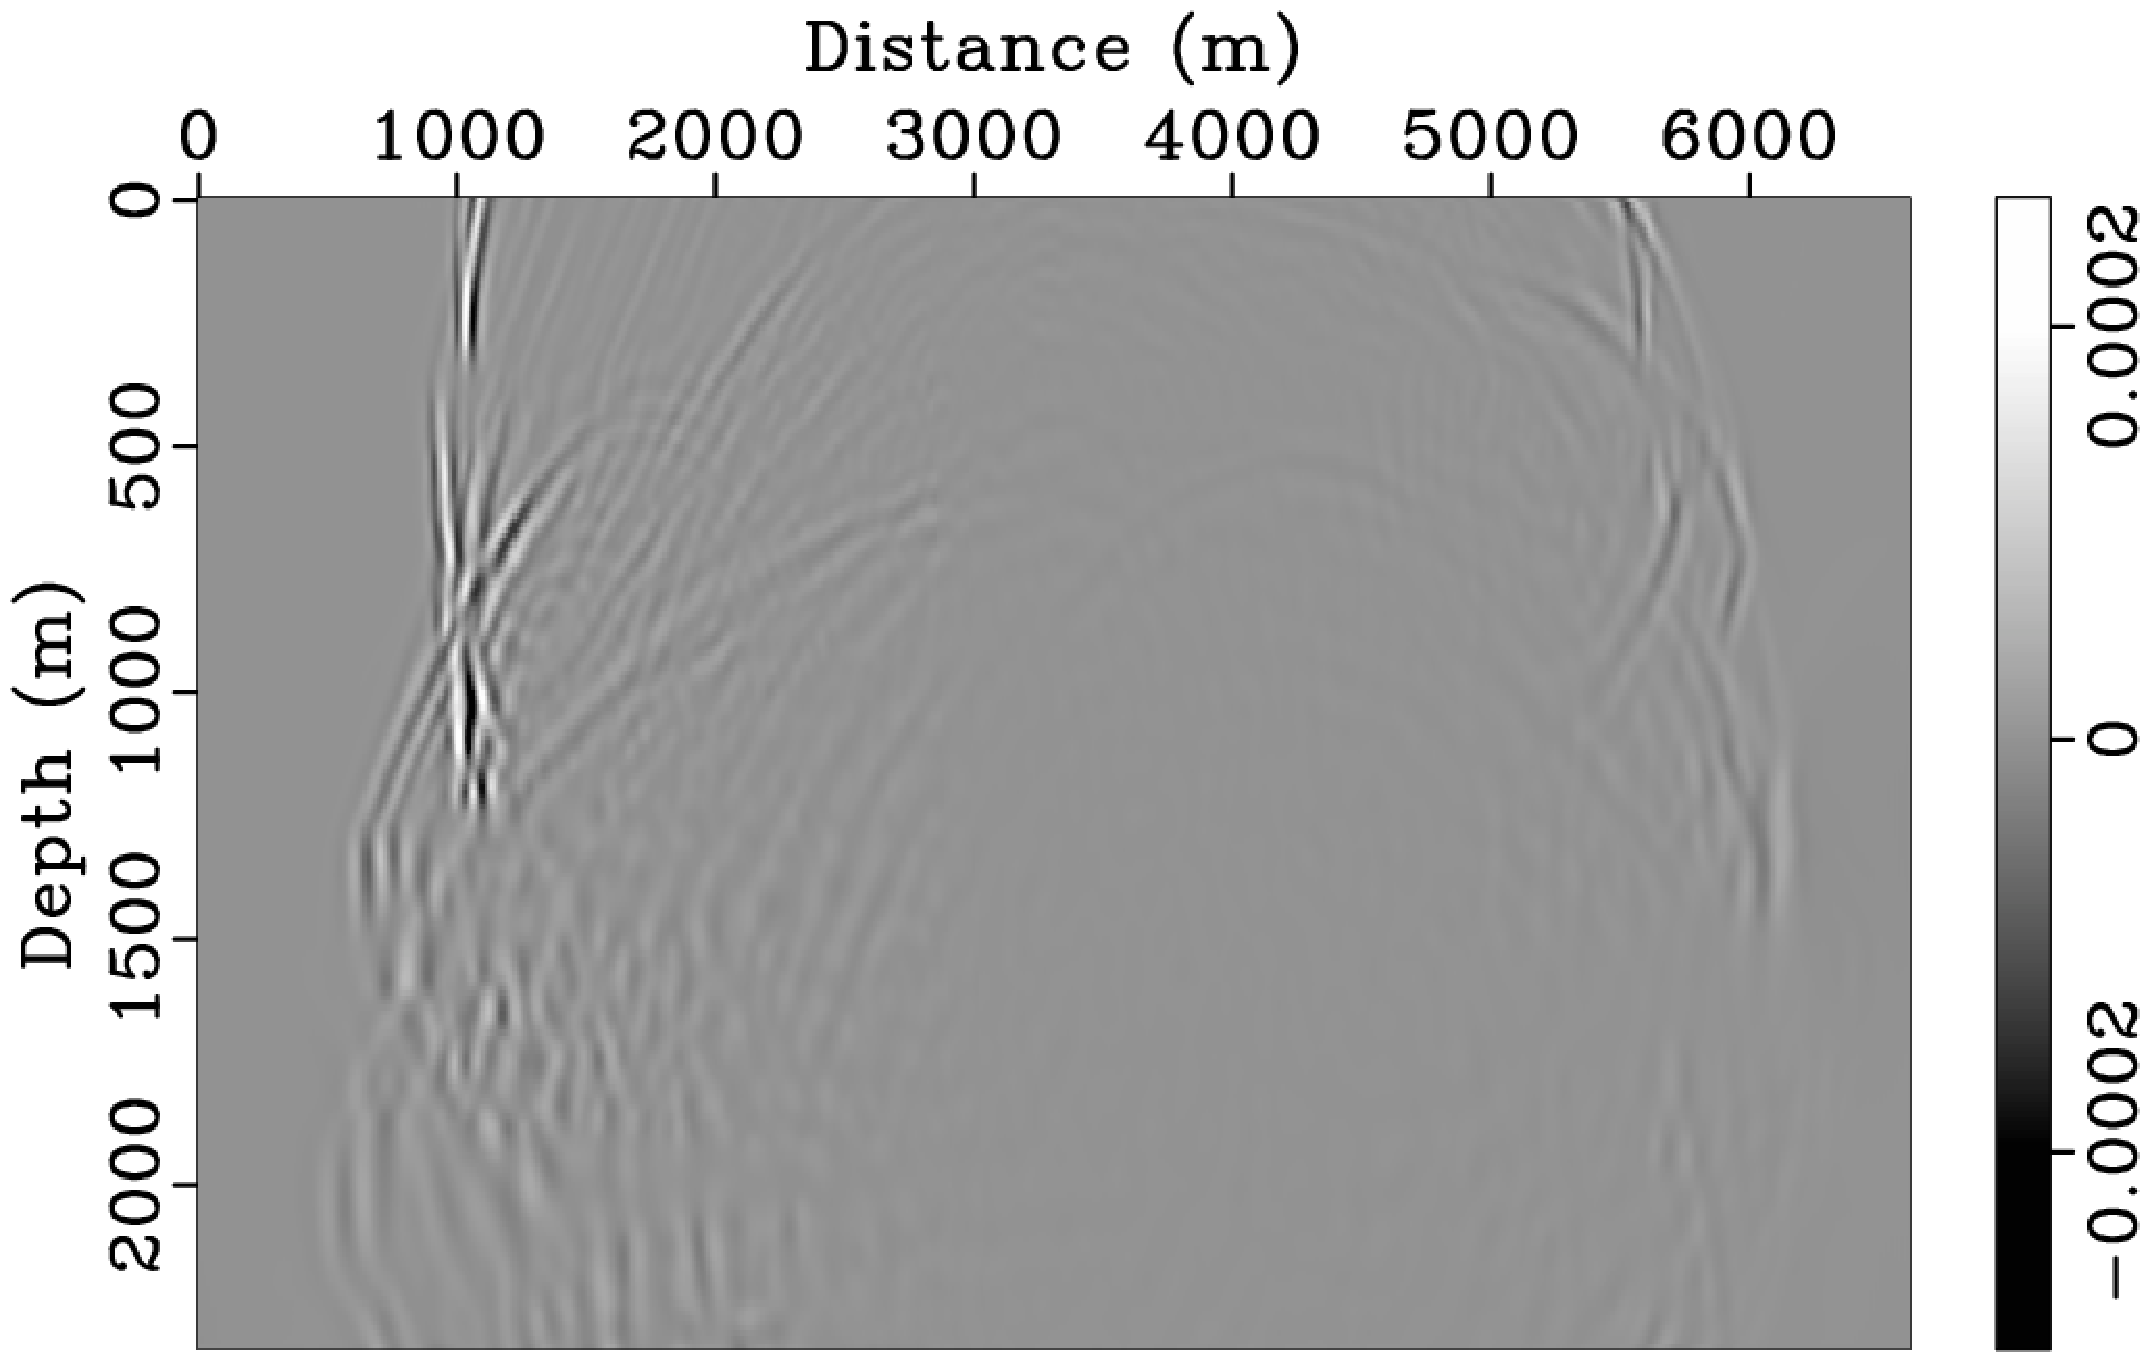
\includegraphics[width=0.3\linewidth]{Fig12f_v.pdf} 
%}
%\caption{Forward snapshots, reconstructed snapshots and their differences from Marmousi model (see Figure \ref{fig:vp,qp}) at two propagation times: (a)-(c) $t=0.82$ s and (d)-(f) $t=1.22$ s. \label{fig:Fig12a_v,Fig12b_v,Fig12c_v,Fig12d_v,Fig12e_v,Fig12f_v}} 
%\end{center} 
%\end{figure}



As this chapter mainly focuses on $Q$-RTM and its GPU implementation, we do not pay much attention to the numerical simulation of spatially varying fractional power of Laplacian operators. There are effective proposed schemes to handle spatial variable-order fractional Laplacians \citep{Sun2014Viscoacoustic, Li2016Efficient, chen2016two, Wangning2018A, wang2018adaptive}. \cite{chen2016two} proposed two efficient methods to calculate spatial variable-order fractional Laplacians, i.e., Taylor-expansion approximation scheme and Low-rank decomposition scheme. \cite{Wangning2018A} extended the Taylor-expansion approximation scheme to the viscoelastic case. All of these methods come at the expense of computational efficiency. In this code package, the averaged strategy \citep{Zhu2014Q} is used to achieve a quick solution. Improving the accuracy of the code package will be my future work.

Another critical issue is the constructed architecture and parallelism strategy of the cu$Q$-RTM code package. The architecture of the cu$Q$-RTM code package has been discussed in detail, which can be separated into four components: memory manipulation, kernel, module and multi-level parallelism. Task-oriented kernels form several fully functional modules, and these modules are further integrated into a complete process of $Q$-RTM. The package contains 2D seismic imaging schemes on both compensated and non-compensated frames with adaptive stabilization and low-pass filtering strategies. We can execute $Q$-RTM in a flexible manner by choosing a series of flags responsible for switching among different scenarios without any code modifications. In this sense, cu$Q$-RTM provides a general GPU-based framework to ensure a time- and memory-efficient implementation. The proposed cu$Q$-RTM is implemented in an MLP manner to take advantages of all the CPUs and GPUs available, while maintaining impressively good stability and flexibility. Whether for a single shot test or a complete simulation, with only a single machine containing seven Nvidia GPU cards, cu$Q$-RTM consistently provides speedup factors approaching or exceeding 50 times compared to conventional CPU-only implementations. My package is particularly well suited to $Q$-RTM where multiple shots are run on clusters with multiple GPUs per node.

Shared memory is expected to be much faster than global memory, which enables direct GPU-to-GPU transfers \citep{nandapalan2012implementation, jaros2012use}. Many researchers proposed shared memory strategy for GPU parallel computing to improve computational efficiency \citep{micikevicius20093d, liu2012fourier, jaros2012use, nandapalan2012implementation, Liu20133D}. In the cu$Q$-RTM code package, we adopt streamed CUFFT to improve computational efficiency with no domain decomposition and GPU-to-GPU transfers involved. For this reason we do not take shared memory strategy into considersation, which might be considered as an improvment in a future version.

Apart from outlining the architecture of the cu$Q$-RTM code package and underlining some program optimization schemes, we also provide speedup analysis and strong scaling test on synthetic models. With only a single Nvidia GPU card, the presented cu$Q$-RTM code package can be 50-80 times faster than the state-of-art distributed CPU implementation running on a single CPU core. We also find that GPU-based simulation on larger model scale tends to reach higher speedup ratio compared with that of small-scale simulation. Objectively speaking, an abusolute speedup ratio without considering the hardware that we used is not really a ``fair'' comparison. In this study, we test the package on a GeForce GTX760 GPU and comapre it with the conventional CPU implementation running on a single core of Intel Core i5-4460 CPU. If a more modern CPU system or a better GPU card is used, the speedup ratio would be much lower or higher than that we claimed in this study. Regarding the scaling test on multi-GPUs, the provided code package exhibits excellent scalability and can be run with almost ideal code performance in part because communications are almost entirely overlapped with calculations. My package's architecture is designed to mimic how a geophysicist writes down a seismic processing module such as modeling, imaging, and inversion. By utilizing the streamed CUFFT, the most time-consuming part of the pseudo-spectral simulation can be computed synchronously on each device, which improves performance and lends itself naturally to the future implementation of more complicated ($Q$-compensated) LSRTM and FWI \citep{Yang2015A, jaros2016full} on the GPU. Future work may also generalize to the 3D case and incorporate more efficient reconstruction scheme, while a further investigation of alternative or improved 2D and 3D FFTs techniques across multiple GPUs \citep{jaros2012use, jaros2016spectral} may also prove worthwhile.  

\section{Summary}

In this chapter, we have presented an open-source code package cu$Q$-RTM, equipped with a set of the state-of-art strategies such as streamed CUFFT, the CATRC scheme, and adaptive stabilization, to achieve an efficient and robust $Q$-RTM. The architecture of the cu$Q$-RTM code package is composed of four components: memory manipulation, kernel, module, and multi-level parallelism. Task-oriented kernels are consolidated into several fully functional modules, which are further integrated into the complete process of $Q$-RTM. The package is implemented in an MLP manner to take advantages of all the CPUs and GPUs available, while maintaining impressively good stability and flexibility. We have demonstrated the effectiveness and applicability of the developed package by performing $Q$-RTM on both synthetic and field data. Either synthetic or field migrated images with $Q$ compensation exhibit sharper reflections and more balanced amplitude. Furthermore, speedup tests via viscoacoustic modeling on layered models indicates that the presented cu$Q$-RTM can be 50-80 times faster, compared with  conventional CPU-based implementation with only a single GPU card. The strong scaling analysis of $Q$-RTM across multiple GPUs demonstrates the excellent scalability of the package.



\bibliographystyle{seg}
\bibliography{qrtm}

\newpage

